
\section{Introduction}%
\label{sec:introduction}

La PMF étant un modèle d'apprentissage statistique, le regroupement des espèces chimiques
en différents facteurs est sensible à la méthodologie employée et au jeu de variable
utilisé.

Les ions et les éléments traces (métaux notamment) permette l'identification de facteur
maintenant bien connus, typiquement : sel de mer, traffic routier, poussière crustale.
Or des questions sont toujours ouvertes pour certains autres facteurs également souvent
identifiés. Les facteurs inorganiques secondaires (nitrate d'amonium et sulfate
d'ammonium) n'ont pas de source bien établie, s'agissant de processus secondaires après
émissions.
Aussi, la pluralité importante des sources de la matière organique et la diversité des
espèces chimiques la composant rendent encore complexe la compréhension des différentes
émissions conduisant à sa présence dans l'atmosphère.

On peut notamment citer quelques espèces organiques ciblant particulièrement certaines sources
(\textit{espèces traceuses}) comme le lévoglucosan pour la combustion de biomasse par
exemple, maintenant utilisé dans de nombreuses études.
D'autres espèces ou groupement d'espèces permettraient également le raffinement des PMF
et depuis plusieurs années, les travaux du groupe essaient d'évaluer la pertinence de
l'ajout de nouveaux traceurs dans les études PMF afin de mieux prendre en compte
certaines émissions anthropiques ou biogéniques mais également afin de mieux estimer la
contribution des aérosols secondaires, qu'ils soient organiques ou inorganique.

De plus, l'identification précise de nouveau facteur diminue l'ambiguité rotationelle
propre à la PMF, et permet donc des solutions plus précise \autocite{emamiEffect2017}.
La recherche de nouvelles espèces traceuses permet donc non seulement d'identifier de
nouvelles sources, mais également de diminuer l'incertitude de celles déjà bien établies.

À ce titre, le site de Grenoble les Frènes a permis le prélèvement et analyse de composés
organiques (HULIS, hopanes, oxy- et nitro-HAP ainsi que oxy- et nitro-HAPS) permettant de
mettre en évidence la saisonalité de ces composés, tracant différent processus : émissions
lié à la combustion en hiver pour les oxy- et nitro-HAP ainsi que leur transport longue
distance alors que les oxy- et nitro-HAPS semblent quant à eux être davantage liés aux
processus d'oxydation secondaires du fait de leur corrélation avec
l'oxalate~\textcite{tomazSources2017a}.

Les rares études incorporants ces traceurs permettent bien l'identification de facteurs
distincts (anthropique secondaire grâce à l'acide phthalic
\autocite{srivastavaSpeciation2018a}, biogénique secondaire grâce à l'oxalate
\autocite{petitSources2019}, traffic routier grâce aux hopanes
\autocite{srivastavaSpeciation2018a}, combustion de biomasse et traffic grâce aux
\ce{^14C}, methoxyphénol et hopanes \autocite{chevrierChauffage2016}, combustion de
charbon grâce aux HAPS \autocite{gollyEtude2014}, etc.).
Cependant, ces études doivent encore être approfondies car trop peu nombreuses et non
reproduite sur un ensemble important de site de mesure. Aussi, certaines de ces espèces ne
sont pas analysées en routines.
Enfin, certaines questions restent ouvertes sur la provenance exacte de certains de ces
composés (MSA, oxalate, glucose…) complexifiant l'interprétation des solutions PMF
obtenue.

Cela est particulièrement vrai pour les réactions secondaires. En effet, par définition
une espèce traceuse est peu réactive, or la matière organique est au contraire très
réactive. Il y a donc une nécessité de travail en amont de l'inclusion dans les études PMF
pour comprendre précisément la dynamique de ces composés dans l'atmosphère, y compris leur
provenance primaire ou secondaire, leur réactivité, etc. 
Notons qu'à ce titre, le couplage entre les différentes méthodes d'analyses, apportant
chacune une vision différente de l'aérosol, est riche d'enseignement (PMF couplant
données AMS, radiocarbon et analyse chimique sur filtre \autocite{vlachouDevelopment2019},
filtre et aethalometre \autocite{chevrierChauffage2016}, chimie et distribution en taille
\autocite{bozzettiSizeResolved2016}, etc.).

Ainsi, la méthodologie d'utilisation du modèle PMF est encore actuellement en évolution,
et ce chapitre discutera des différentes avancées ou pistes que ma thèse a exploré ces
dernières années.

\section{Validation externe des solutions PMF}%
\label{sec:confrontation_des_solutions_pmf}

Comme discuter précédemment, un modèle doit être évalué par des mesures externes. Or, il
est compliqué voire impossible de « mesurer » la concentration des sources de PM (c'est
justement le travail demandé à la PMF). On ne peut donc faire que des confrontations
indirectes, à travers d'autres types de mesure ou modèle, chimique ou géophysique, afin
d'estimer la fiabilité d'une solution PMF.

\subsection{Confrontation aux mesures de radiocarbone \ce{^{14}C}}%
\label{sub:14c}

Sur les sites de la vallée de l'Arve dans le cadre du programme DECOMBIO, en plus des mesures
traditionnelles sur filtre, \textcite{bonvalotEstimating2016} ont également estimé par
traçage isotopique au radiocarbone \ce{^{14}C} l'origine fossile ou récente du carbone.
Les études PMF sur le site de Passy et Chamonix de \textcite{chevrierChauffage2016},
illustrées figure~\ref{fig:chapter03/radiocarbon_chevrier_winter} ont
montrées une très bonne concordance entre la quantité de carbone provenant de source
fossile estimée par radiocarbone et les facteurs PMF traçant des sources de combustion de
carbone fossile. Réciproquement, le carbone récent est en très bon accord entre les mesures
radiocarbone et PMF.

Cette confrontation à des mesures externes à la PMF conduisant à des résultats concordant
accentue fortement la confiance que l'on peut avoir dans les résultats et la
quantification de la contribution des sources issues de ces analyses.

\begin{figure}[ht]
    \centering
    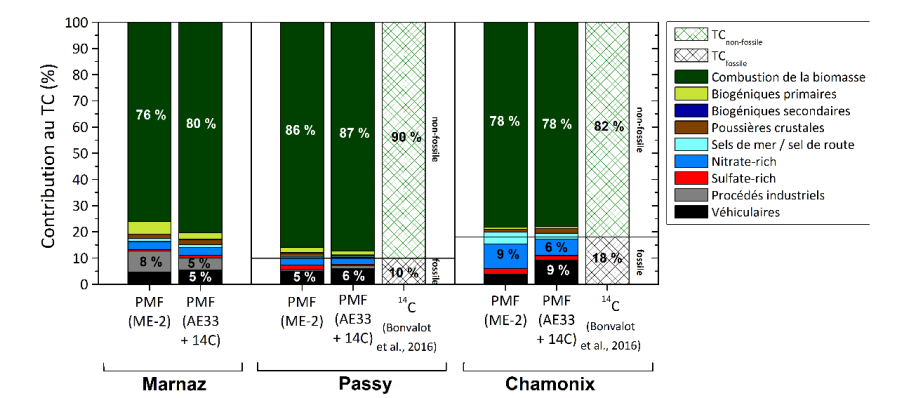
\includegraphics[width=1.0\linewidth]{chapter03/radiocarbon_chevrier_winter.png}
    \caption{Contributions relatives au carbone total en moyennes hivernales des sources
        de \PMdix{} identifiées lors de la thèse de \textcite{chevrierChauffage2016} par les
        différentes approches PMF et contributions des parts fossile et non-fossile
        obtenues par l’analyse du radiocarbone de \textcite{bonvalotEstimating2016}.
    Source: \textcite[figure 75]{chevrierChauffage2016}}%
    \label{fig:chapter03/radiocarbon_chevrier_winter}
\end{figure}

\subsection{Confrontation mesure sur site récepteur et origine géographique}%
\label{sub:confrontation_mesure_sur_site_recepteur_et_origine_geographique}

Les facteurs PMF étant déterminés au niveau du site recepteur mais n'étant pas
nécessairement émis à cet endroit spécifique, il est également possible d'estimer leur
provenance géographique et leur vraisemblance. Nous verrons d'abord le cas simple de la
rose des polluants, avant d'expliciter plus en avant la méthode PSCF.

\subsubsection{Cas simple : la rose des polluants}%
\label{ssub:cas_simple_la_rose_des_polluants}

\begin{tcolorbox}[colback=red!5!white,colframe=Melon,title=Note]
    Utiliser à des fins exploratoires lors de ma thèse, j'ai contribué au développement
    du module python \href{https://github.com/python-windrose/windrose/}{windrose},
    récemment publiée~\autocite{scls19frPythonwindrose2019}.
\end{tcolorbox}

L'un des moyens les plus simples pour cela est de coupler des mesures de direction et
vitesse de vent et d'établir une rose des polluants, projetant sur un graphique en
coordonnée polaire la concentration des polluants suivant la direction en $\theta$ et
vitesse du vent en $r$ au moment de l'observation.

Cependant, cette méthode n'est utile que pour la détermination de source proche du site
récepteur car dès lors que l'on s'en éloigne, l'orientation et vitesse des vents varient
et l'hypothèse de déplacement uniforme de la masse d'air est invalidée.  Or, il est
courant que les aérosols proviennent de sources non locales, limitant l'utilisabilité de
cette méthode.


\subsubsection{Prendre en compte l'histoire de la masse d'air : PSCF}%
\label{sub:prendre_en_compte_l_histoire_de_la_masse_d_air_PSCF}

\begin{tcolorbox}[colback=red!5!white,colframe=Melon,title=Note]
    Ces étapes fastidieuses de calcul des rétrotrajectoires et de PSCF ont été automatisés
    dans un paquet python, pyPSCF\footnote{Dépôt git pyPSCF:
    \url{https://gricad-gitlab.univ-grenoble-alpes.fr/webersa/pyPSCF}}, permettant le
    traitement d'un grand nombre de rétrotrajectoires en utilisant le modèle lagrangian
    HYSPLIT et calculant de manière facilitée une PSCF en un site donné, en variant
    notamment les différents paramètres susceptibles d'influencer le modèle.

    Également, et de manière similaire à ZeFir de \cite{petitUserfriendly2017}, pyPSCF
    propose une interface utilisateur permettant une interaction facilité.
\end{tcolorbox}

Pour s'affranchir de la limitation des roses des vents, il est possible d'utiliser les
rétrotrajectoires complètes des masses d'air pour remonter aux sources géographiques
potentielles, mais également de coupler ces trajectoires à des informations
physico-chimiques comme la concentration en polluants observés sur le site récepteur, la
présence de pluie sédimentant les aérosols par dépôt humide ou encore la hauteur de la
masse d'air.

L'une des méthodes les plus largement utilisées dans la littérature est la \textit{Potential
source contribution function} (PSCF), permettant de combiner des ensembles de trajectoires à
des modèles récepteurs. Le principe consiste à calculer les rétrotrajectoires d'un site
récepteur donné et d'associer à chacune d'elle la concentration du polluant ou de la
source considéré le jour de son passage au niveau du site récepteur. En discrétisant les
trajectoires en 1 point toutes les X minutes ou heures et en appliquant une grille
régionale, il est alors possible de dénombrer combien de rétrotrajectoires sont passés par
chacune des grilles.  Le ratio du nombre de trajectoire associée à une forte concentration
aux coordonnées $i$, $j$, noté $m_{ij}$, par le nombre total de trajectoire étant passé
par ces coordonnées notées $n_{ij}$, nous donne une probabilité de provenance géographique
de ce composé ou source pour les coordonnées $i$, $j$, noté $PSCF_{ij}$ :
\begin{align}
    \label{eq:PSCF}
    PSCF_{ij} &= \frac{m_{ij}}{n_{ij}}.
\end{align}

Des améliorations ont été apportées à cette méthode afin de prendre en compte les cellules
ayant un faible pourcentage de passage de rétrotrajectoires, augmentant artificiellement
le ratio $\frac{M}{N}$. Une manière de contrebalancer ce biais et d'ajouter une fonction
poids, dépendant de la fréquence de passage des rétrotrajectoires sur chacune des
cellules. Dans la figure~\ref{fig:chapter02/PSCF_method}, illustrant la PSCF, on voit que
la cellule où 2 rétrotrajectoires sont passés se voit attribuer la même probabilité que
celles avoisinantes, où seule une rétrotrajectoire a résidé. Or, il serait plus pertinent
d'avoir une probabilité plus forte pour cette cellule, indiquant que chaque
rétrotrajectoire ayant résidé à ces coordonnées est riche du composé suivit.  Différentes
fonctions poids existent, le plus souvent présentant différents seuils en fonction du
nombre de rétrotrajectoires par cellule~\autocite{bressiSources2014,petitSources2019}.

Aussi, pour avoir une représentativité statistique suffisante des sources potentielles, il
est nécessaire de calculer un grand nombre de rétrotajectoires, correspondant à chacun des
jours de prélèvement sur le site récepteur.

\begin{figure}[ht]
    \centering
    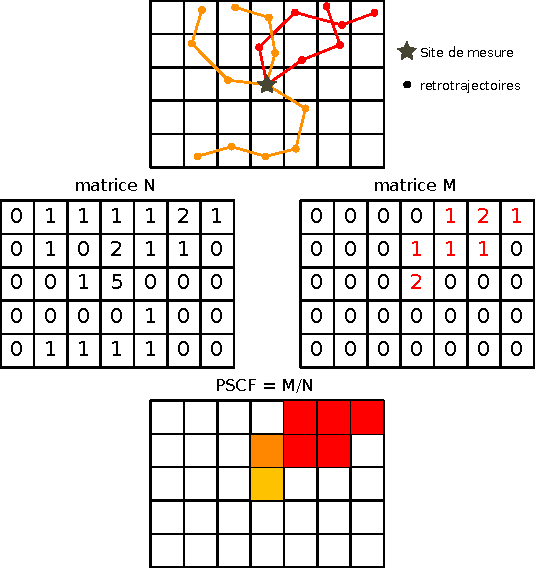
\includegraphics[width=0.9\linewidth]{chapter03/PSCF_method.pdf}
    \caption{Illustration de la méthode PSCF : les rétrotrajectoires depuis le site de
        mesure sont calculées, celles associées à une concentration seuil sont
        représentées en rouge, les autres en orange. Les matrices N et M s'obtiennent par
        simple décompte du nombre de rétrotrajectoires passés dans chaque cellule de
        taille prédéfinies, puis le ratio nous donne une estimation de l'origine
    géographique, représentée ici terme d'intensité de rouge.}%
    \label{fig:chapter02/PSCF_method}
\end{figure}

\subsubsection{Application de la PSCF}%
\label{ssub:application_de_la_pscf}

\begin{tcolorbox}[colback=red!5!white,colframe=Melon,title=Note]
Cette partie synthétise dans un premier temps les résultats de~\cite{gollyOrganic2019},
dans lesquels mon implication a porté notamment sur le calcul et l'analyse PSCF, et dans
un second temps expose l'une des méthodes de validation possible des PMF grâce aux PSCF,
appliquée sur le site de l'OPE.
\end{tcolorbox}

\paragraph{Importance et origine géographique du MSA}%
\label{par:origine_terrestre_ou_marine_du_msa_}

Comme expliqué précedemment, une part importante des aérosols provient de sources
secondaires, c'est-à-dire du vieillissement et des réactions dans l'atmosphère. Une part
importante de ces aérosols secondaires sont d'origines organiques. Les travaux
de~\textcite{gollyOrganic2019}, s'attachent notamment à la quantification de cette matière
organique secondaire sur 5 sites ruraux en France pendant l'année 2013, par la mesure de
deux espèces issues de processus secondaires : le MSA et l'oxalate.  Nous avons pu montrer
que le MSA, considéré comme provenant de l'oxydation du DMS, peut contribuer jusqu'à 10 à
20\% de l'OC en période chaude, indiquant une forte proportion d'aérosols organiques
secondaires durant l'été. Mais surtout, le MSA est considéré comme provenant des émissions
de DMS du phytoplancton marin, au point qu'il est proposé comme méthode de séparation
entre le sulfate d'origine marine et ses autres provenances.

En conduisant une analyse PSCF sur les 25\% des jours les plus fortement chargés en MSA
sur les 5 sites, nous avons pu confirmer l'importance marine de ce composé. 
Cependant, une part non négligeable semble également provenir d'environnement terrigène (voir
figure~\ref{fig:chapter03/golly_PSCF_MSA}), confortant les études suggérant des processus
d'émissions du MSA par des sources biologiques terrestres~\autocite{bozzettiArgon2017},
pouvant provenir des forêts ou des
sols~\autocite{jardineDimethyl2015,miyazakiSeasonal2012}.

L'une des implications directes de ces travaux résulte en l'ajout systématique du MSA
comme variable d'entrée des études PMF, quels que soient leurs localisations. En effet, le
signal du MSA est clairement distinct des autres espèces chimiques mesurées et représente
également une part important de la matière organique. Cette espèce est donc a minima
traceuse de processus secondaires présents sur l'ensemble de l'Europe occidentale.

\begin{figure}[ht!]
    \centering
    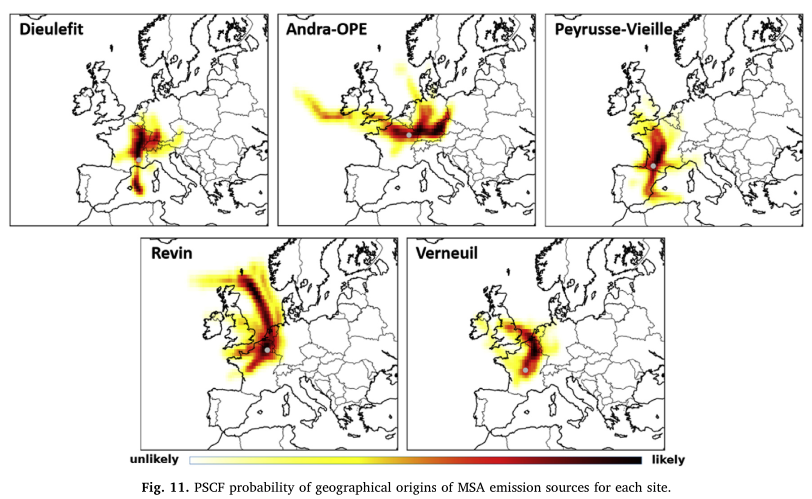
\includegraphics[width=0.9\linewidth]{chapter03/golly_PSCF_MSA.png}
    \caption{Probabilité de l'origine géographique du MSA, issue de l'article
        de~\textcite{gollyOrganic2019}. Bien que l'on retrouve l'origine marine du MSA,
        les sites de Dieulefit, OPE ou Peyrusse-Vieille indiquent également une forte
        probabilité d'origine terrestre de ce composé.}%
    \label{fig:chapter03/golly_PSCF_MSA}
\end{figure}

\paragraph{Confrontation PSCF -- PMF}%
\label{par:confrontation_pscf_pmf}

Une autre utilisation de la PSCF consiste à croiser les informations issues de la PSCF et
des PMF.
En effet, il n'existe pas de moyen simple de valider le sens géochimique d'une solution
PMF autrement que l'expertise et les connaissances de l'utilisateur.

Pour estimer la fiabilité de la solution obtenue, il est possible de conduire une
étude PSCF sur les différents facteurs identifiés. On s'attend à ce que le
facteur \textit{sel de mer} provienne géographiquement d'un océan ou d'une mer par
exemple.

Un exemple d'utilisation de ce procédé est expliqué et illustré dans la section dédiée aux
PMF et isotopie, section~\ref{sub:isotopie}.



\section{Incertitudes associées aux PMF}%
\label{sub:incertitudes_associées}

Le modèle PMF est maintenant relativement couramment utilisé dans le domaine de la
qualité de l'air. Seulement, peu d'étude rapportent en même temps que leur solution
finale, les incertitudes associées. Or, le solveur ME-2 permet l'estimation de ces
incertitudes à travers les méthodes de bootstrap et de displacment (voir
section~\ref{par:incertitudes}).

Seulement, ces incertitudes ne sont rapportées par l'EPAPMF5.0 que pour les concentrations
des espèces chimiques des différents facteurs et non pour leurs contributions temporelles.
Notamment, leur de l'estimation de la variabilité via bootstrap, les différents facteurs
sont attribués aux facteurs de références d'après leur corrélation temporelle (par défaut
$r > 0.6$), mais seuls les profils chimiques sont rendu à l'utilisateur par la suite.
Une solution serait de manuellement explorer 100 solutions PMF, avec ou sans tirage
aléatoire des échantillons, pour estimer respectivement la variabilité provenant du modèle
statistique ou de la représentativité du jeu de donnée. Malheureusement, cette
répétabilité est beaucoup trop fastidieuse à faire à la main et ne peut pas s'automatiser à
partir de l'EPAPMF5.0. Or, il s'agit de l'implémentation du ME-2 la plus largement
utilisée. C'est pourtant un besoin important lors de la transférabilité de nos recherches
vers l'opérationnel, avec des questions très pratiques cherchant l'incertitude
sur la contribution de telle source pour tels jours de pic de pollution en particulier.

Une «astuce» consiste alors à réestimer la variabilité des contributions temporelles
$X_{err}$ à partir de la variabilité de la composition chimique des profils, i.e. en gardant
$G$ fixe (celle de référence, $G_{ref}$) mais en utilisant les profils $F_{err}$ issue
des bootstraps et ambiguïté rotationelle :
\begin{align}
    \label{eq:hack_unc}
    X_{err} &= G_{ref} \times F_{err}.
\end{align}

Même si en théorie pour la méthode du bootstrap à la fois $G$ et $F$ doivent
évoluer en même temps, cela donne une première estimation de la gamme d'incertitude pour
chaque espèce et chaque jour d'observation.

Cette visualisation, présentée à titre d'exemple pour la PMF de Vif
figure~\ref{fig:chapter03/vif_nitraterich_all} permet de rapidement se rendre compte du
type d'incertitude prépondérant pour chacune des espèces (représentativité de
l'échantillonnage et ambiguïté rotationelle) mais également de la gamme de valeur possible
pour chaque jour étant donnée les incertitudes estimées.

\begin{figure}[ht]
    \centering
    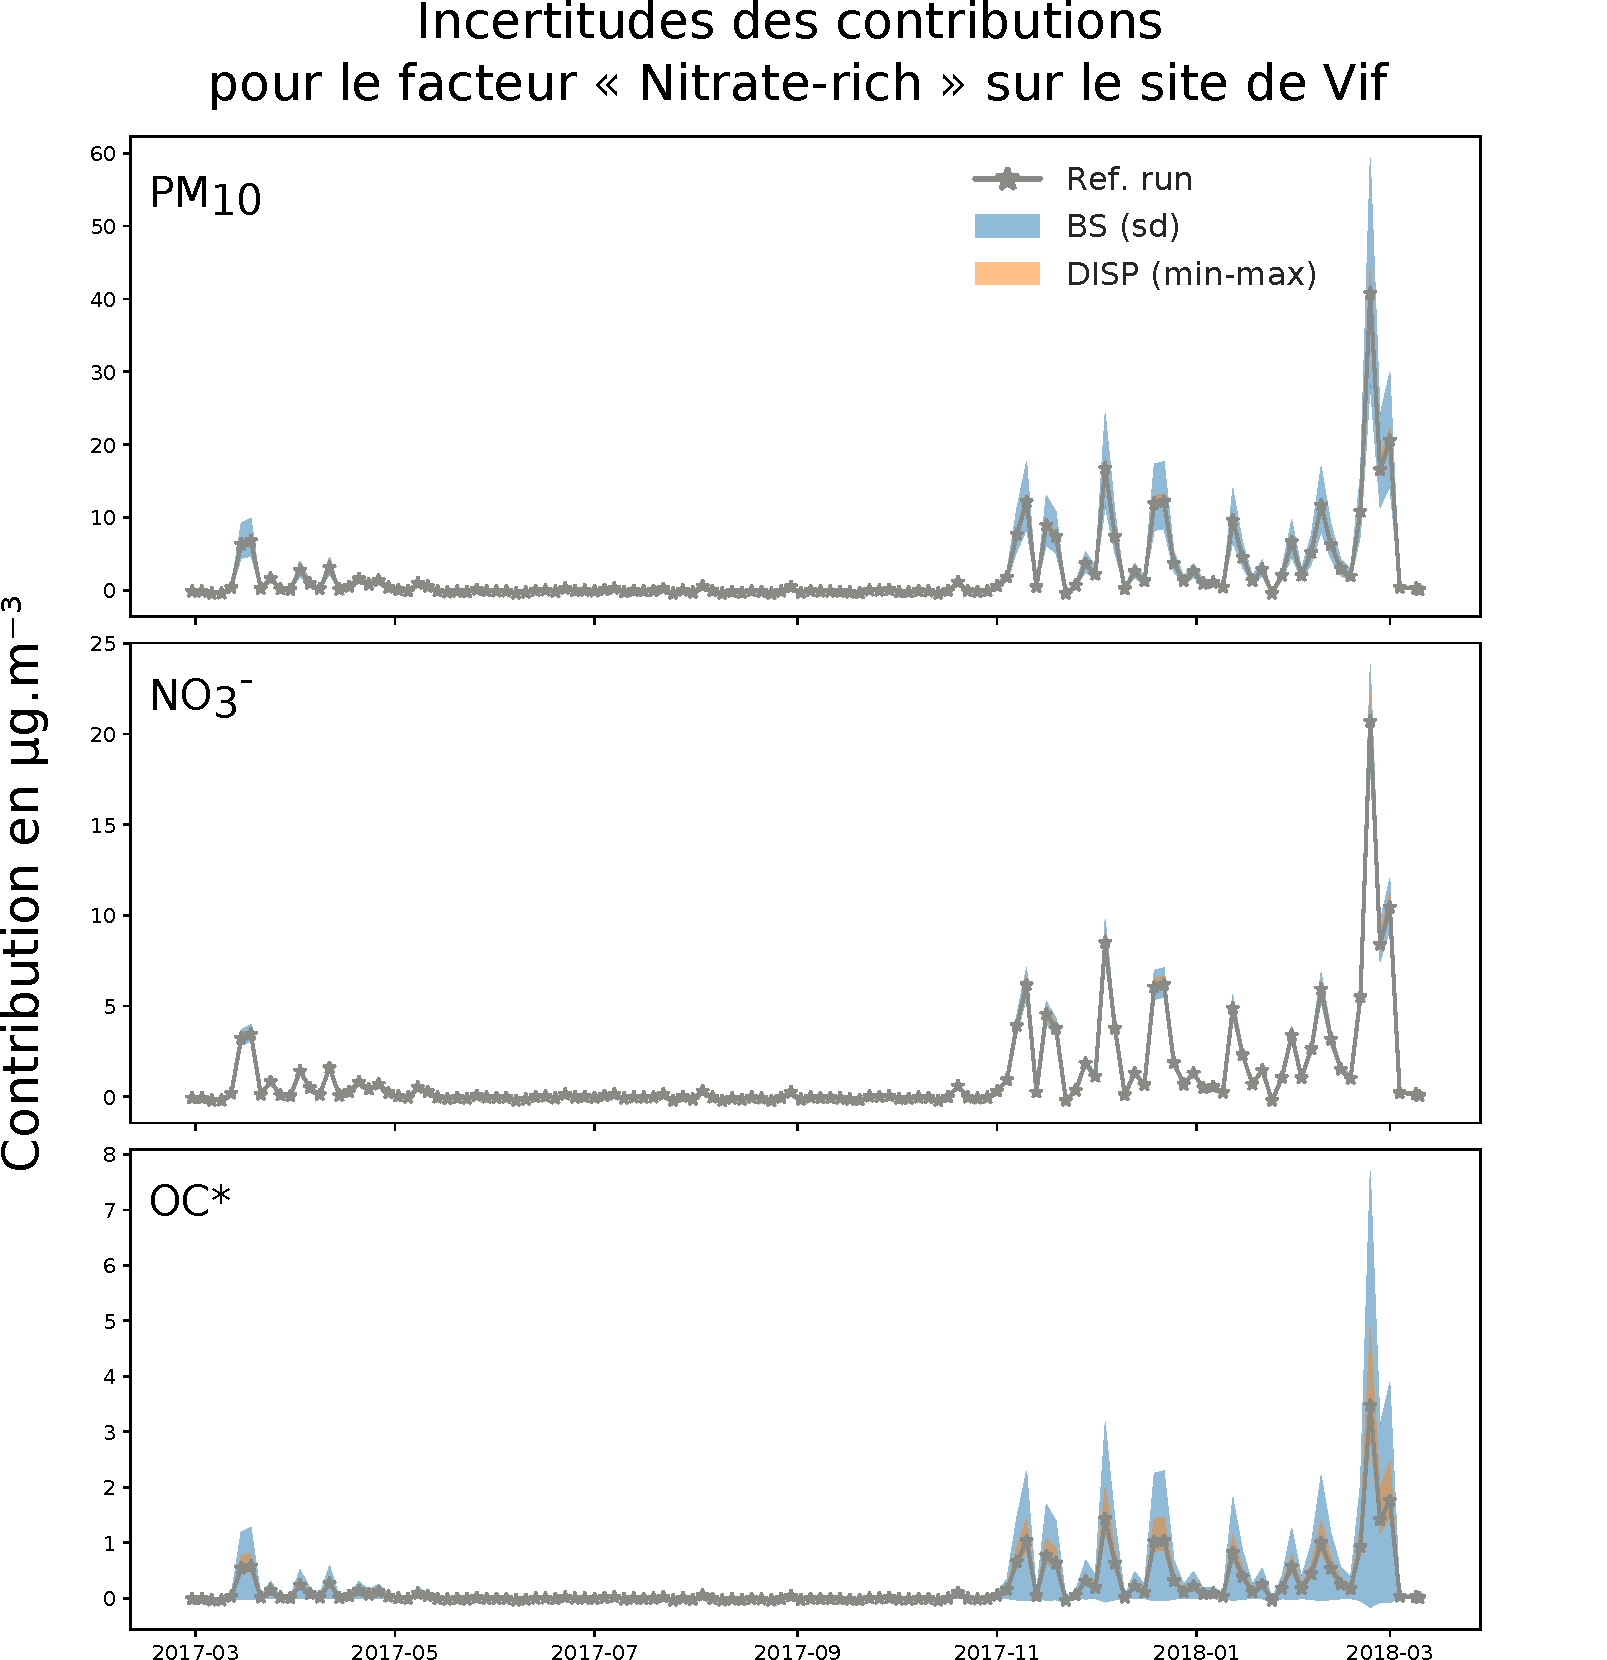
\includegraphics[width=0.8\linewidth]{chapter03/vif_nitraterich_all.pdf}
    \caption{Incertitudes temporelles des concentrations de \PMdix, \NOt et OC* dans le
        facteur Nitrate-rich de Vif estimé par boostrap (écart type de 100 bootstraps en bleu)
        et displacment (min et max en orange). La solution de référence est représenté par les
    traits et étoiles grises.}%
    \label{fig:chapter03/vif_nitraterich_all}
\end{figure}


\section{Comparabilité des solutions}%
\label{sub:comparabilité_des_solutions}

Une problématique récurrente lors de l'utilisation des PMF est de se demander si les
profils que l'on obtient seraient nommés de la même façons par d'autres utilisateurs, et
si oui, comment peut-on évaluer la proximité géochimique de facteurs identiquement nommés
en différents endroits (spatiallement ou temporellement).

Les travaux de \cite{belisNew2015a} suggèrent l'utilisation conjointe de 2
métriques permettant d'estimer la distance géochimique entre 2 profils de facteurs.

\subsection{Méthodologie}%
\label{sub:méthodologie}

\paragraph{Distance de Pearson}%
\label{par:distance_de_pearson}

La distance de Pearson (\textit{Pearson distance} PD) estime la proximité entre 2 série de
donnée en utilisant leur corrélation de Pearson, soit :
\begin{align}
    \label{eq:PD}
    PD &= 1 - r^2
\end{align}
avec $r$ la corrélation entre les 2 séries de données. Pour les profils chimiqes des
facteurs, il s'agit de la concentration relative des espèces chimiques les constituants
(i.e. pourcentage massique de chacune des espèces).

Seulement, cette distance est très sensible aux extrêmes du fait de sa dépendance au
coefficient de correlation. Ainsi, si seul l'OC est similaire pour les 2 profils mais la
totalité des métaux présentent des concentrations très différentes, alors le PD pourra
être acceptable car l'OC présente des concentrations relative bien supérieure à celles
des métaux (voir figure~\ref{fig:chapter03/PD_belis2015a}).
De plus, la distance de Pearson ne teste que l'hypothèse de relation linéaire entre les
deux profils, et non leur égalité stricte.

\begin{figure}[ht]
    \centering
    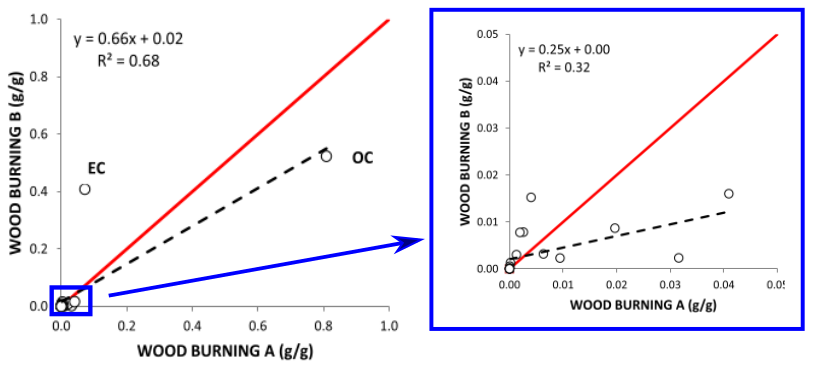
\includegraphics[width=1.0\linewidth]{chapter03/PD_belis2015a.png}
    \caption{Mesure de la distance de pearson de 2 sources \textit{wood burning}. L'image
        de droite montre l'influence des espèces dominant la masse pour le calcul du PD, alors
        qu'en leur absence, le PD change drastiquement (image de droite). Source: adapté de
        \cite[figure 3]{belisNew2015}.
}%
    \label{fig:chapter03/PD_belis2015a}
\end{figure}


\paragraph{Distance identitaire standardisée}%
\label{par:distance_identitaire_standardisée}

Pour répondre aux problèmes soulevés par la distance de Pearson, \textcite{belisNew2015}
propose l'utilisation de la distance identitaire standardisée (\textit{Standardized
Identity Distance} SID). Sa formulation a légèrement évoluée entre son expression
initiale par \textcite{belisNew2015} et celle actuellement utilisée par SPECIEUROPE
\autocite{pernigottiSPECIEUROPE2016,pernigottiDeltaSA2018}.

L'idée principale consiste à exprimer la distance entre chaque pair d'espèce $i$ pour les 2
profils considérés $x$ et $y$ et la droite unitée, noté $ID_i$ pour \textit{identity
distance}, telle que:
\begin{align}
    \label{eq:IDi}
    ID_i &= \frac{1}{\sqrt{2}}|x_i - y_j|.
\end{align}
Aussi, afin de prendre en compte de manière homogène toutes les espèces et s'extraire du
biais sur-considérant les espèces prépondérantes à la masse, l'ID est normalisée par une
valeure proportionnelle à la moyenne de la masse de l'espèce $i$ dans le facteur $x$ et
$y$, appelée \textit{maximum acceptable distance} MAD, telle que:
\begin{align}
    \label{eq:MAD}
    MAD_i &= k \frac{1}{2}(x_i + y_i).
\end{align}
Ce procédé est illustré figure~\ref{fig:chapter03/SID_belis2015a}.

La SID est la moyenne de la somme des ratios entre l'ID et le MAD, telle que:
\begin{align}
    \label{eq:SIDi}
    SID &= \frac{1}{m}\sum_i^m\frac{ID_j}{MAD_j},
\end{align}
soit :
\begin{align}
    \label{eq:SID}
    SID &= \frac{\sqrt{2}}{km} \sum_i^m \frac{|x_i - y_i|}{x_i + y_i}.
\end{align}

\begin{figure}[ht]
    \centering
    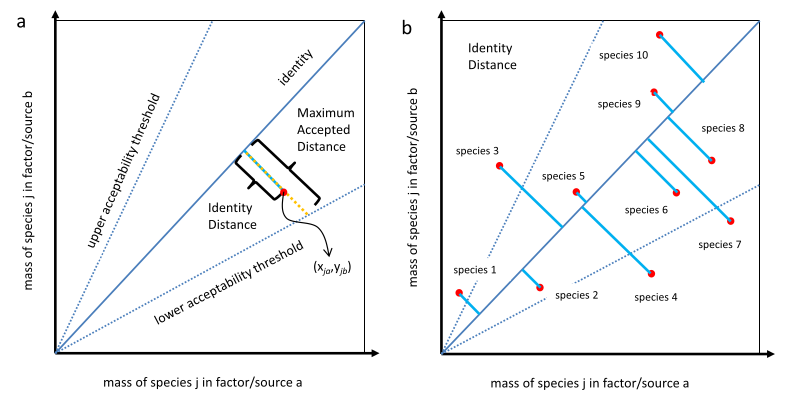
\includegraphics[width=0.9\linewidth]{chapter03/SID_belis2015a.png}
    \caption{Illustration schématique de la distance SID. Légende originelle:
        Geometric representation of the identity distance (ID) as an indicator of
        similarity between two factor/source profiles. Left pane: $ID_{j,ab}$ between
        factor/sources $a$ and $b$ for species $j$ with acceptability thresholds (dotted lines);
        the dot represents point ($x_{ja}$, $y_{jb}$ ). Right pane: comparison of two
        hypothetical factor/sources with 10 common species.
        Source: \cite[figure 2]{belisNew2015}
}%
    \label{fig:chapter03/SID_belis2015a}
\end{figure}

\subsection{Implémentation et utilisation}%
\label{sub:implémentation_et_utilisation}

Ces 2 métriques de distances entre profils sont utiles pour l'aide à l'identification
d'un nouveau profils, notamment via SPECIEUROPE. Cependant, toutes les espèces chimiques
que nous utilisons «en routine» ne sont pas nécessairement présente dans les profils de
SPECIEUROPE. Aussi, SPECIEUROPE nous permet de comparer aux profils déjà existant, et non
par exemple des PMF sur 2 sites non encore dans la base de donnée SPECIEUROPE.

Ainsi, pour comparer les profils chimiques issues d'une même méthodologie PMF (même
variables d'entrée, même contraintes, etc) à différents lieux, j'ai ré-implémenté une version
de deltaTool en python\footnote{Disponible dans le paquet
    \href{https://pypi.org/project/py4pm/}{py4pm}, dépot git:
\url{https://gricad-gitlab.univ-grenoble-alpes.fr/webersa/py4pm}
} permettant une
utilisation plus flexible et une comparabilité des PMF étudiées pendant ma thèse.

Le choix de $k$ de l'Eq.~\ref{eq:SID} pour le MAD a été porté à 1, similairement à
\cite{pernigottiDeltaSA2018}, en absence d'information a priori sur la variabilité de ces
profils.

La question de la comparabilité des profils s'est posé majoritairement à 3 moments de ma
thèse :
\begin{enumerate}
    \item Comparer 15 PMF utilisant une méthodologie harmonisée en France (projet SOURCES);
    \item Étudier la variabilité fine échelle (i.e. à l'échelle d'une métropole) à travers
        3 sites de prélèvement dans un rayon de \SI{15}{\kilo\m} autour de Grenoble, France
        (projet Mobil'Air);
    \item Évaluer l'impact de l'ajout de traceurs organiques (acide pinique, phthalique,
        3-MBTCA et cellulose) par rapport à une PMF «standard» sur les 3 sites
        Grenoblois (projet Mobil'Air).
\end{enumerate}

Le premier item sera abondamment traité dans la section~\ref{sec:sources} et
\textcite{weberComparison2019}, tandis que les 2 autres font l'objet d'un article en
cours de soumission par \textcite{borlazaFinescaleinprep.} et sont détaillés succinctement
dans la section~\ref{sub:processus_secondaires}.

\section{Amélioration des solutions PMF par ajout de traceurs spécifiques}%
\label{sec:amélioration_des_solutions_pmf}

\subsection{Apport de l'isotopie de l'azote sur la caractérisation des sources de pollution émettrices d’ammonium}%
\label{sub:isotopie}

Les résultats présentés dans cette partie sont en partie issus d'un travail antérieur à ma
thèse dans l'équipe CHIANTI dans le cadre du projet INACS de l'ADEME portant sur
la caractérisation des épisodes de pollutions printanier au nitrate d'ammonium.

\begin{tcolorbox}[colback=red!5!white,colframe=Melon,title=Note]
    Ces travaux ont été présentés dans le rapport INACS-2 (présenté en
    annexe~\ref{annexe:INACS}) et lors d'une présentation orale à l'EAC de Tours en 2016
    \autocite{weberNitrogen5}.
    Un article est également en cours d'écriture sur ce sujet.  Les principales méthodes
    et résultats sont repris dans cette section.
\end{tcolorbox}

\begin{tcolorbox}[colback=red!5!white,colframe=ProcessBlue,title=Note]
    Certaines valeurs ne sont pas identiques entre le rapport et celles présentées içi
    car ces travaux ont continué et certains paramètres ont changé entre la publication
    du rapport et l'écriture de la thèse.
\end{tcolorbox}


\subsubsection{Problématique}%
\label{ssub:problématique}

Dans de nombreuses PMF, il est rapporté un facteur secondaire inorganique contennant une
grande part du sulfate, du nitrate et de l'ammonium, indiquant la présence de sulfate
d'ammonium \ce{SO4(NH4)2} et nitrate d'ammonium \ce{NO3NH4}. Ces deux facteurs sont
également souvent distincts, formant un facteur «sulfate rich», présentant le sulfate
d'ammonium mais sans nitrate, et «nitrate rich» présentant du nitrate d'ammonium mais
sans sulfate.

Le facteur \textit{Nitrate-rich} présente des émissions très saisonnière, responsable des grands
événements de dépassement des seuils d'alerte printanier. Seulement, s'agissant d'un
facteur secondaire issu de condensation des NOx et de l'ammoniac \ce{NH3}, sa provenance
n'est pas clairement établi. En effet, si les NOx sont supposés venir du traffic routier,
la provenance de l'ammoniac peut aussi bien être agricole via l'urée ou les fertilisants de
synthèse que liée au trafic routier. Aussi, une source importante émettant pendant les
pics de pollution pourrait être la combustion de biomasse domestique, notamment en vallées
alpines, où cette source est active et corrélée au nitrate d'ammonium au début du printemps.

\subsubsection{Objectifs et méthode}%
\label{ssub:objectif_et_methode}

L'isotopie est une technique connue permettant l'estimation des sources d'émission,
seulement, il n'est pas possible de l'utiliser tel quel dans une analyse PMF et donc
d'avoir cette information pour identifier plus précisément la source nitrate rich.
En effet, la PMF résout une équation d'équilibre des masses et est donc purement
additive. Or, l'isotopie se traduit par une équation de mélange, résultant en une moyenne
pondérée de la signature isotopique des sources par leurs contributions.

Par contre, s'il n'est pas possible d'inclure directement le signal isotopique dans les
PMF, il est possible d'effectuer un traitement en amont de la PMF, permettant de séparer
l'ammonium ou le nitrate en différentes « sous espèces », selon leurs sources de
provenances, grâce à l'isotopie.

Dans ce cadre, le programme INACS de l'ADEME a permis les mesures de l'isotopie de l'azote
du nitrate et de l'ammonium sur des cycles annuel complet à X sites.  Parallèlement, les
mesures de la signature isotopique à l'émission de différentes sources ont été faites,
notamment en tunnel et à l'émission de cheminée (combustion de biomasse domestique), ainsi
que de substances issues de sources agricoles (fumier, fertilisant de synthèse, bâtiment
d'élevage, etc).

L'ensemble de cette étude est disponible en annexe \ref{annexe:INACS} et ne sont présentés
ci-après que les étapes et résultats majeurs de cette étude.

\paragraph{Équation de mélange}%
\label{par:équation_de_mélange}

La première partie du programme INACS a montré que ces sources présentent des signatures
isotopiques de l'azote distincte pour l'ammoniac, noté \dN(\NHq).
Nous pouvons alors, sous certaines conditions, proposer une déconvolution de l'équation de mélange
\begin{align}
    \dN(\NHq)_{atm} \cdot [NH_4^+]_{atm} &= \sum_{i=1}^{n} \dN(\NHq)_i \cdot [NH_4^+]_i
    \label{eq:melangeConcentration}
\end{align}
avec $[NH_4^+]_{atm} = \sum_{i=1}^n [NH_4^+]_i$ [\si{\ugm}] la concentration atmosphérique
d'ammonium résultant du mélange des $n$ sources.  L'équation~\ref{eq:melangeConcentration}
peut être réécrite en considérant $f_i = [NH_4^+]_i / [NH_4^+]_{atm}$~[-] comme étant la
contribution de la source $i$ au mélange final. Ainsi on a
\begin{align}
    \dN(\NHq)_{atm} &= \sum_{i=1}^n \dN(\NHq)_i \cdot f_i. 
    \label{eq:melangeContrib}
\end{align}

Selon certaines hypothèses, détaillées dans l'annexe~\ref{annexe:INACS}, en considérant les
trois sources précédemment citées supposées majoritaires, à savoir combustion de biomasse,
agricole et véhiculaire, pour chaque observation de \dN(\NHq)$_{atm}$ le système
d'équation~\ref{eq:system1} suivant doit alors être vérifié :
\begin{numcases}{\label{eq:system1}}
    1 &$= f_{bio} + f_{agr} + f_{veh}$ \label{eq:bilanMass1} \\
    \dN(\NHq)_{atm} &$= f_{bio} \cdot \dN(\NHq)_{bio} + f_{agr} \cdot \dN(\NHq)_{agr} + f_{veh} \cdot \dN(\NHq)_{veh}$ \label{eq:systemNH4}
\end{numcases}
où $f_{bio}$, $f_{agr}$ et $f_{veh}$ sont respectivement la contribution de la source de
biomasse, agricole et véhiculaire et $\dN(\NHq)_{bio}$, $\dN(\NHq)_{agr}$ et
$\dN(\NHq)_{veh}$ les compositions isotopiques respectives des sources biomasse, agricole
et véhiculaire.

\paragraph{Résolution par méthode Monte-Carlo}%
\label{par:résolution_par_méthode_monte_carlo}

La signature isotopique des sources étant connues avec une incertitude, l'équation de
mélange est résolue par méthode Monte-Carlo : pour chaque jour d'observation, l'équation
\ref{eq:systemNH4} est résolue pour un triplet de valeur possible de chacune des
signatures isotopiques des 3 sources, suivant une loi normale établit par la moyenne et
l'écart type de chacun des prélèvements de ces sources. Le processus est répété 1000 fois
pour chaque jour d'observation, résultat ainsi en 1000 triplets $(f_{agr}, f_{bio},
f_{veh})$ possibles, permettant de calculer la concentration et l'incertitude associée de
l'ammonium apporté par chacune de ces sources.

\paragraph{Ajout d'une contrainte pour l'ammonium issu de la combustion de biomasse}%
\label{par:ajout_d_une_contrainte_pour_l_ammonium_issu_de_la_combustion_de_biomasse}

\subparagraph{Nécessité d'une nouvelle contrainte}%
\label{par:nécessité_d_une_nouvelle_contrainte}

Le système d'équation \ref{eq:system1} est sous-déterminée : il existe 3 inconnues pour
seulement 2 contraintes (bilan de masse et isotopie). De fortes incertitudes sont donc
attendues, voir des concentrations calculées seront invraisemblables, notamment pour les
concentrations de la combustion de biomasse.
Deux nouvelles contraintes pourraient être ajoutées pour ajouter de l'information et
réduire le degré de liberté du système : 1) une information sur l'isotopie de l'hydrogène
et 2) une connaissance \textit{a priori} de la géochimie des sources.  La deuxième
solution est retenue.  En effet un proxy de la combustion de biomasse, le lévoglucosan,
est déjà mesuré pour la quasi-totalité des sites d'études.

\subparagraph{Concentrations de lévoglucosan et d'ammonium}%
\label{par:concentrations_de_lévoglucosan_et_d_ammonium}

De par le recensement en une base de donnée unique de la filtrothèque de l'équipe
CHIANTI (voir \ref{sec:harmonisation_et_gestion_de_base_de_donnée}), il a été possible
d'estimer empiriquement des gammes de concentrations possible pour l'ammonium en fonction
des concentrations en lévoglucosan. Puisque les vallées alpines sont connues pour présenter
des épisodes de pollutions aux particules fines dont la source est quasi exclusivement
la combustion de biomasse \autocite{piotAtmospheric2011,gollyEtude2014} et que le lévoglucosan
est considéré comme traceur univoque de la combustion de biomasse, en utilisant les
données chimiques de ces sites, il est possible de trouver une relation entre la
concentration de \NHq~issue de la combustion de biomasse et la concentration en
lévoglucosan. 

Le seuil de concentration en lévoglucosan à \SI{5000}{\ugm} est considéré comme critère de
sélection des jours où la source biomasse est prépondérante. 
Pour ces jours-ci, le \NHq~émis est considéré comme provenant de la combustion de
biomasse.
Avec ces hypothèses, une régression linéaire entre l'ammonium et le lévoglucosan montre la
relation $[\NHq] = 0.221 \times \text{[levoglucosan]}$ (trait plein sur la
figure~\ref{fig:correlNH4Levo}).
L'écart-type est volontairement choisi très large pour rendre compte du faible nombre
d'échantillon (18) et du caractère expérimental de cette relation (trait pointillés sur la
figure~\ref{fig:correlNH4Levo}).

Ainsi, l'équation suivante est ajoutée au système à résoudre
\begin{numcases}{\label{eq:system3}}
    f_{bio} &$= \{\mathcal{N}(m_{bio},\sigma_{bio})\}$ / [\NHq$_{total}$] \label{eq:bioChimie}\\
    1 &$= f_{bio} + f_{agr} + f_{veh}$ \label{eq:bilanMasse}\\
    \dN(\NHt)_{atm} &$= f_{bio} \cdot \dN(\NHt)_{bio} + f_{agr} \cdot \dN(\NHt)_{agr} + f_{veh} \cdot \dN(\NHt)_{veh}$\label{eq:isotopie}.
\end{numcases}
L'équation~\ref{eq:bioChimie} étant une contrainte a priori et non isotopique. 
Elle réduit la liste des valeurs théoriquement possibles, tandis que
l'équation~\ref{eq:isotopie} sélectionne celles qui sont en accords avec l'observation
isotopique.

\begin{figure}[ht]
    \centering
    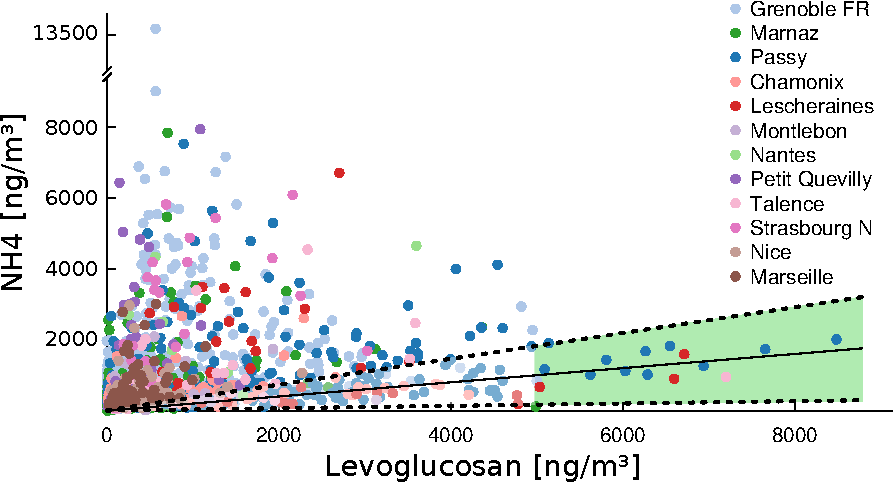
\includegraphics[width=0.7\textwidth]{figures/INACS/MCA_correlNH4Levo_alea.pdf}
    \caption{Estimation du ratio \NHq/lévoglucosan pour les jours de fortes concentrations en
        lévoglucosan. La droite noire en trait plein représente la droite $[\NHq_{bio}]=
        0.221 \times \text{[lévoglucosan]}$, les droites en trait pointillés les
        écart-types considérés ($\frac{1}{8}\times \text{[lévoglucosan]}$) et la zone
        verte les jours où la source de combustion de biomasse est considérée comme
        prépondérante ([lévoglucosan] > \SI{5000}{\ugm}]).
    }
    \label{fig:correlNH4Levo}
\end{figure}

\subsubsection{Détermination des sources de \NHq}%
\label{ssub:determination_des_sources_de_NHq}

\paragraph{Importance de la source agricole pour le \NHq}%
\label{par:importance_de_la_source_agricole_pour_le_nhq}

Le site rural de l'OPE est un site typique des tendances générales de l'ensemble des sites
d'études.
Il est donc utilisé comme illustration dans la suite, pour des prélèvements s'étalant sur
l'année 2013.

Durant la période chaude (de mai à septembre) le fond atmosphérique est très
majoritairement dû au secteur véhiculaire qui explique à lui seul 90$\pm$8~\% du
\NHq~total (\textit{cf.} figure~\ref{fig:timeSerieOPE}.a).
La quantité d'ammonium apportée par cette source est sensiblement constante autour
\SI{0.6(4)}{\ugm} tout au long de l'année (figure~\ref{fig:timeSerieOPE}.b).

D'après le modèle, les épisodes de printemps (mars et avril) sont imputables
majoritairement à la source agricole, qui apporte en $80\pm10$~\% du \NHq~ces jours-ci.
Ce secteur apporte jusqu'à \SI{5}{\ugm} d'ammonium le 2 avril, soit plus de 8 fois
l'apport moyen du véhiculaire.

\begin{figure}[ht]
    \centering
    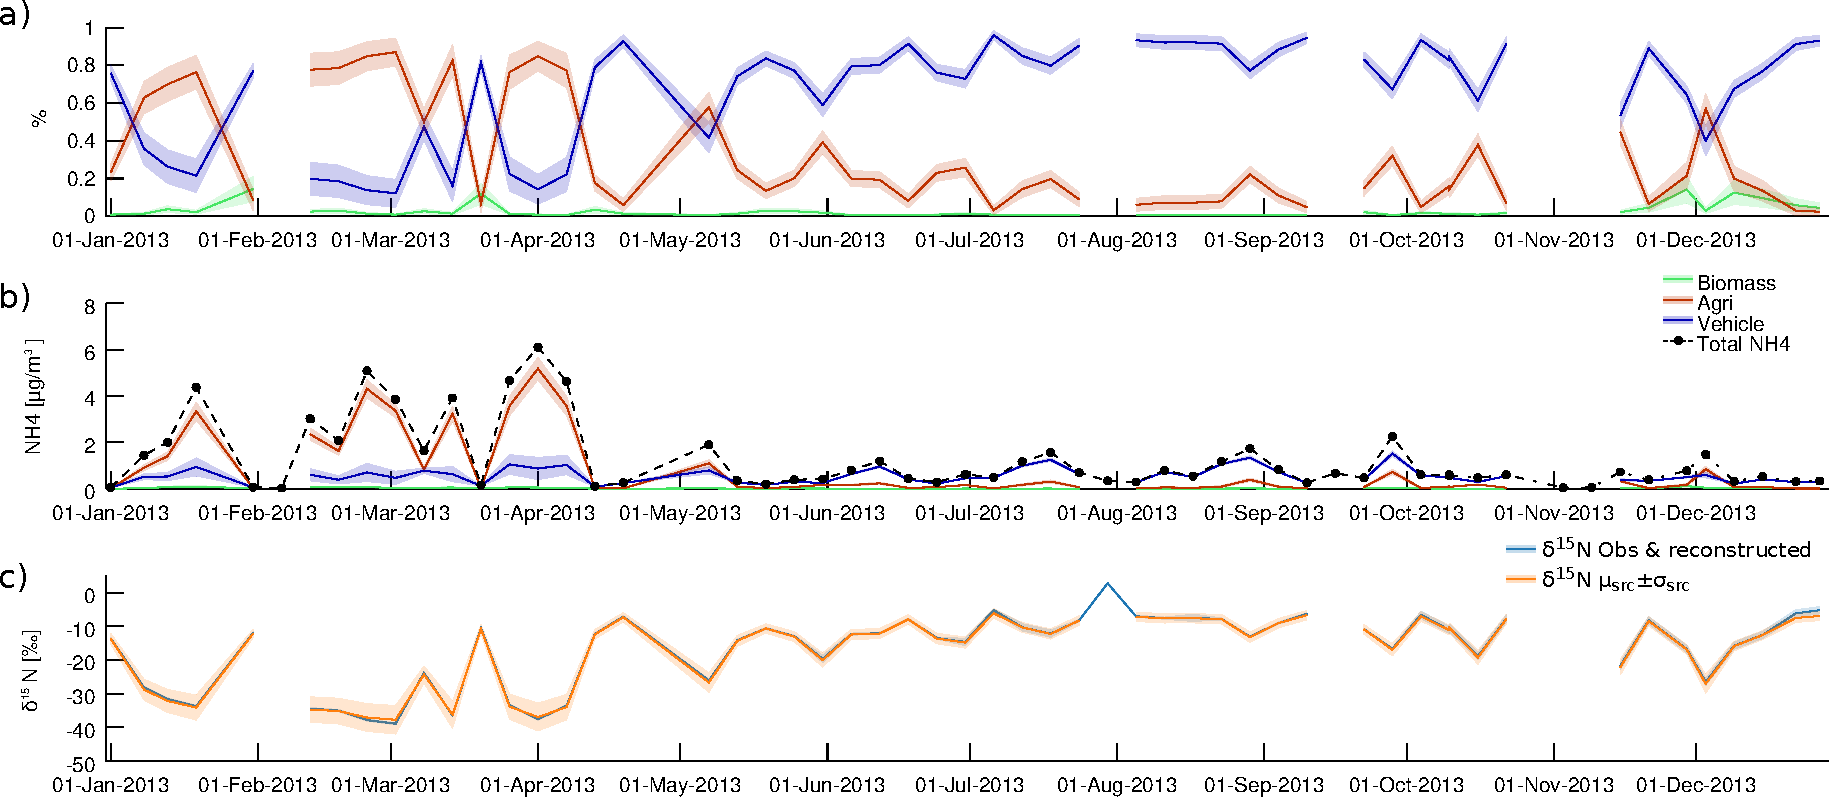
\includegraphics[width=1.0\linewidth]{figures/INACS/MCA_OPE_S3-BioFerVeh_e-30_timeSerie2013.pdf}
    \caption{Série temporelle du site de l'OPE. Sont représentés la moyenne de la densité
        de probabilité et l'écart-type (1$\sigma$) associé. \textbf{a)} Contribution
        relative de chaque source à l'observation. \textbf{b)} Contribution absolue de
        chaque source. Le trait noir pointillé est le \NHq~observé. \textbf{c)}
        \dN~observé et reconstruit en bleu, \dN~reconstruit à partir de la totalité des
        valeurs des sources possibles en oranges.
    }
    \label{fig:timeSerieOPE}
\end{figure}

\paragraph{Fond atmosphérique de l'ensemble des sites}
L'été, lorsque seule la source véhiculaire est active, la même quantité d'ammonium est
observé sur l'ensemble des sites comme le montre la figure~\ref{fig:summerNH4}.
La source véhiculaire est donc sensiblement constante sur l'ensemble du territoire à
raison de $\sim0.6$~\si{\ugm}.
Toutefois les sites de Lens et de Turin semblent être au-dessus de ces tendances, et sont
discutés en annexe \ref{annexe:INACS}.

\paragraph{Épisodes synchrones à l'échelle du territoire}
Sur les sites étudiés, il apparait également que les pics de pollution sont synchrones à
l'échelle nationale : février 2012, février 2013 et mars 2013.
La plupart des pics de pollution lors de ces événements sont attribués pour une grande
part au secteur agricole.
La contribution du \NHq$_{agr}$ au \NHq~total lors de ces épisodes est reportée sur la
figure~\ref{fig:contribSpringAgr}.

Les sites où l'influence du facteur agricole est la plus marquée sont les deux sites
ruraux de Revin et l'OPE pour lesquels les jours les plus impactés sont attribués à plus
de 80~\% à l'agriculture pour des concentrations excédent respectivement 7 et 5
\si{\ugm}, soit environ 10 fois plus que le fond atmosphérique.

\begin{figure}[ht]
    \begin{subfigure}[t]{0.5\textwidth}
    \begin{center}
    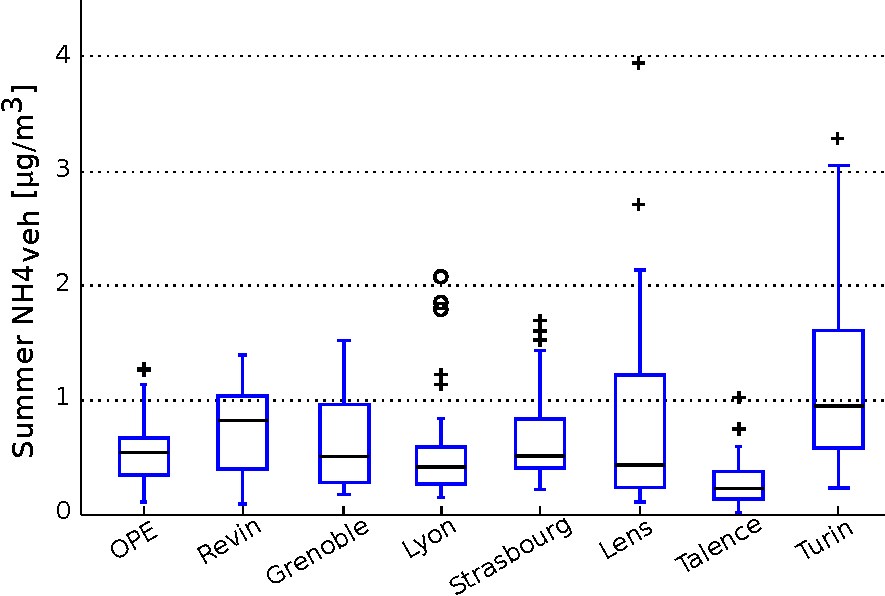
\includegraphics[width=.9\textwidth]{figures/INACS/MCA_contribSummerVeh.pdf}
    \end{center}
    \caption{Contribution moyenne de la source véhiculaire durant les jours de la période chaude.}
    \label{fig:summerNH4}
    \end{subfigure}
    \begin{subfigure}[t]{0.5\textwidth}
    \begin{center}
    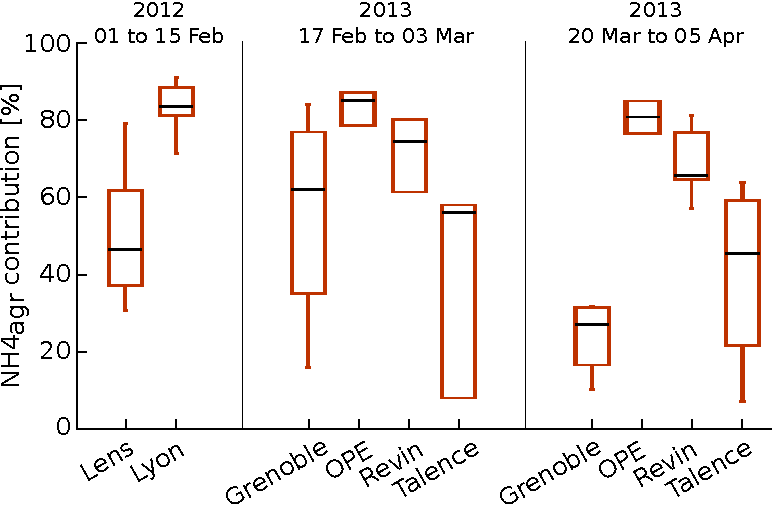
\includegraphics[width=.9\textwidth]{figures/INACS/MCA_contribSpringEventAgr.pdf}
    \end{center}
    \caption{Contribution relative moyenne de la source agricole pour les jours des trois
    pics de pollution printaniers observés.}
    \label{fig:contribSpringAgr}
    \end{subfigure}
    \caption{Contribution des sources véhiculaire et agricole.}
\end{figure}

\subsubsection{Utilisation couplée de l'isotopie et des PMF}%
\label{ssub:utilisation_couplée_de_l_isotopie_et_des_pmf}

\paragraph{Paramètrage de la PMF et solution de référence}%
\label{par:paramètrage_de_la_pmf_et_solution_de_référence}

Une fois le \NHq~séparé en trois variables distinctes cette information peut être utilisée
dans une approche de type Positive Matrix Factorization (PMF) pour mieux comprendre la
dynamique des différents facteurs.
L'avantage majeur de l'utilisation de la PMF sera aussi de faire le lien entre les sources
du nitrate d'ammonium et les sources de PM.

Sur le site de l'OPE a été choisi pour tester la méthodologie car une étude PMF intégrant
les données chimiques de 2012 à 2014 pour la fraction \PMdc{} a déjà été conduite sur ce
site, offrant un comparatif intéressant pour le couplage isotopie/PMF. C'est donc ce site
qui est retenu.

Les variables utilisées sont donc les mêmes que celles de l'étude précédente
de~\cite{gollyCaracterisation2015} auxquelles s'ajoute le chlore et sont rappelées dans le
tableau~\ref{tab:varPMF}.
Pour l'étude couplée chimie et isotopie, seul diffère le \NHq~qui est séparé en trois
espèces \NHq$_{bio}$, \NHq$_{agr}$ et \NHq$_{veh}$. 

\begin{table}[ht]
    \centering
    \footnotesize
    \begin{tabular}{r P{2cm} P{1.5cm} P{5.0cm} P{3.0cm}}
        \toprule
                    & Matière carbonée       &   Métaux      &   Ions                                                &   Composés organiques \\
        \midrule
        PMF         & OC, EC                  & As, Pb, Ti, V & MSA, \NOt, \SOq, Oxalate, \ce{K+}, \ce{Na+}, \ce{Cl-}, \ce{Ca^2+}, \ce{Mg^2+}, \NHq   & Lévoglucosan, $\sum$polyols, HAP \\
        \midrule
        PMF + MC    & OC, EC                  & As, Pb, Ti, V & MSA, \NOt, \SOq, Oxalate, \ce{K+}, \ce{Na+}, \ce{Cl-}, \ce{Ca^2+}, \ce{Mg^2+}, \NHq$_{bio}$, \NHq$_{agr}$, \NHq$_{veh}$ & Levoglucosan, $\sum$polyols, HAP \\
        \midrule
        Incertitudes& Élargie (10~\%, 15~\%)  & \multicolumn{3}{P{10cm}}{Méthode proposée par \cite{gianiniSource2013}, sauf pour les trois \NHq$_{src}$ où $\sigma_{src}/4$ est utilisé.}\\
        \bottomrule
    \end{tabular}
    \caption{Espèces chimiques sélectionnées comme variables d'entrée dans les PMF la pour
    fraction \PMdc.}
    \label{tab:varPMF}
\end{table}

\paragraph{Solution obtenue}%
\label{par:solution_obtenue}

En substituant le \NHq~par ses trois contributions \NHq$_{src}$ dans la PMF, il n'y a pas
de changement significatif pour les facteurs ne présentant pas déjà du \NHq (Secondaire
organique, Sels de mer, Sels de mer vieilli, Biogénique marin et Poussières/Biogénique
primaire).

Le \NHq$_{bio}$ se retrouve bien dans le facteur de combustion de biomasse à raison de
70~\% du \NHq$_{bio}$ total.
Ce résultat était attendu car par construction le modèle Monte-Carlo introduit une
dépendance forte entre le lévoglucosan et le \NHq$_{bio}$.
Il est également intéressant de voir que \textit{seul} l'ammonium issu de la combustion
de biomasse se retrouve dans ce facteur.
Il faut cependant noter que le \NHq$_{bio}$ n'est pas entièrement attribué à ce facteur
mais également au facteur \og Nitrate rich \fg{} (20~\%) et dans un moindre mesure au sel
de mer vieilli (10~\%).

La source Industrie/traffic se voit attribuer 45~\% de l'ammonium dit véhiculaire.
De plus aucune des deux autres sources d'ammonium n'est présente dans ce facteur, ce qui
tend à accentuer l'étiquette \og traffic \fg{} de ce facteur.
Une autre observation importante concerne l'activité de cette source au long de l'année :
l'industrie et le trafic sont connus pour avoir une activité constante, ou du moins non
saisonnière.
Or en n'utilisant pas les données isotopiques deux pics étaient observés fin février et
fin mars.
L'utilisation de l'isotopie diminue l'importance de ces pics, qui étaient
vraisemblablement une erreur d'attribution du \NHq~entre le \NHq$_{veh}$ et le
\NHq$_{agr}$.

Une part non négligeable de l'ammonium dit véhiculaire est également retrouvée dans le
facteur Secondaire organique (>20~\%).
Il serait intéressant d'investiguer plus en avant cet ammonium afin de savoir s'il s'agit
véritablement d'ammonium véhiculaire.

Enfin, le résultat sans doute le plus important réside dans l'identification du facteur
\og Nitrate rich \fg, où la quasi-intégralité (>90~\%) de l'ammonium agricole se retrouve.
Or il n'existe pas à notre connaissance une autre source ayant une signature isotopique
voisine ou plus négative en \dN~que la source agricole.
Ainsi, il n'y a pas d'ambiguïté de source possible et le facteur \og Nitrate rich \fg{}
peut être identifié et renommé Agriculture.

\begin{figure}[ht]
    \centering
    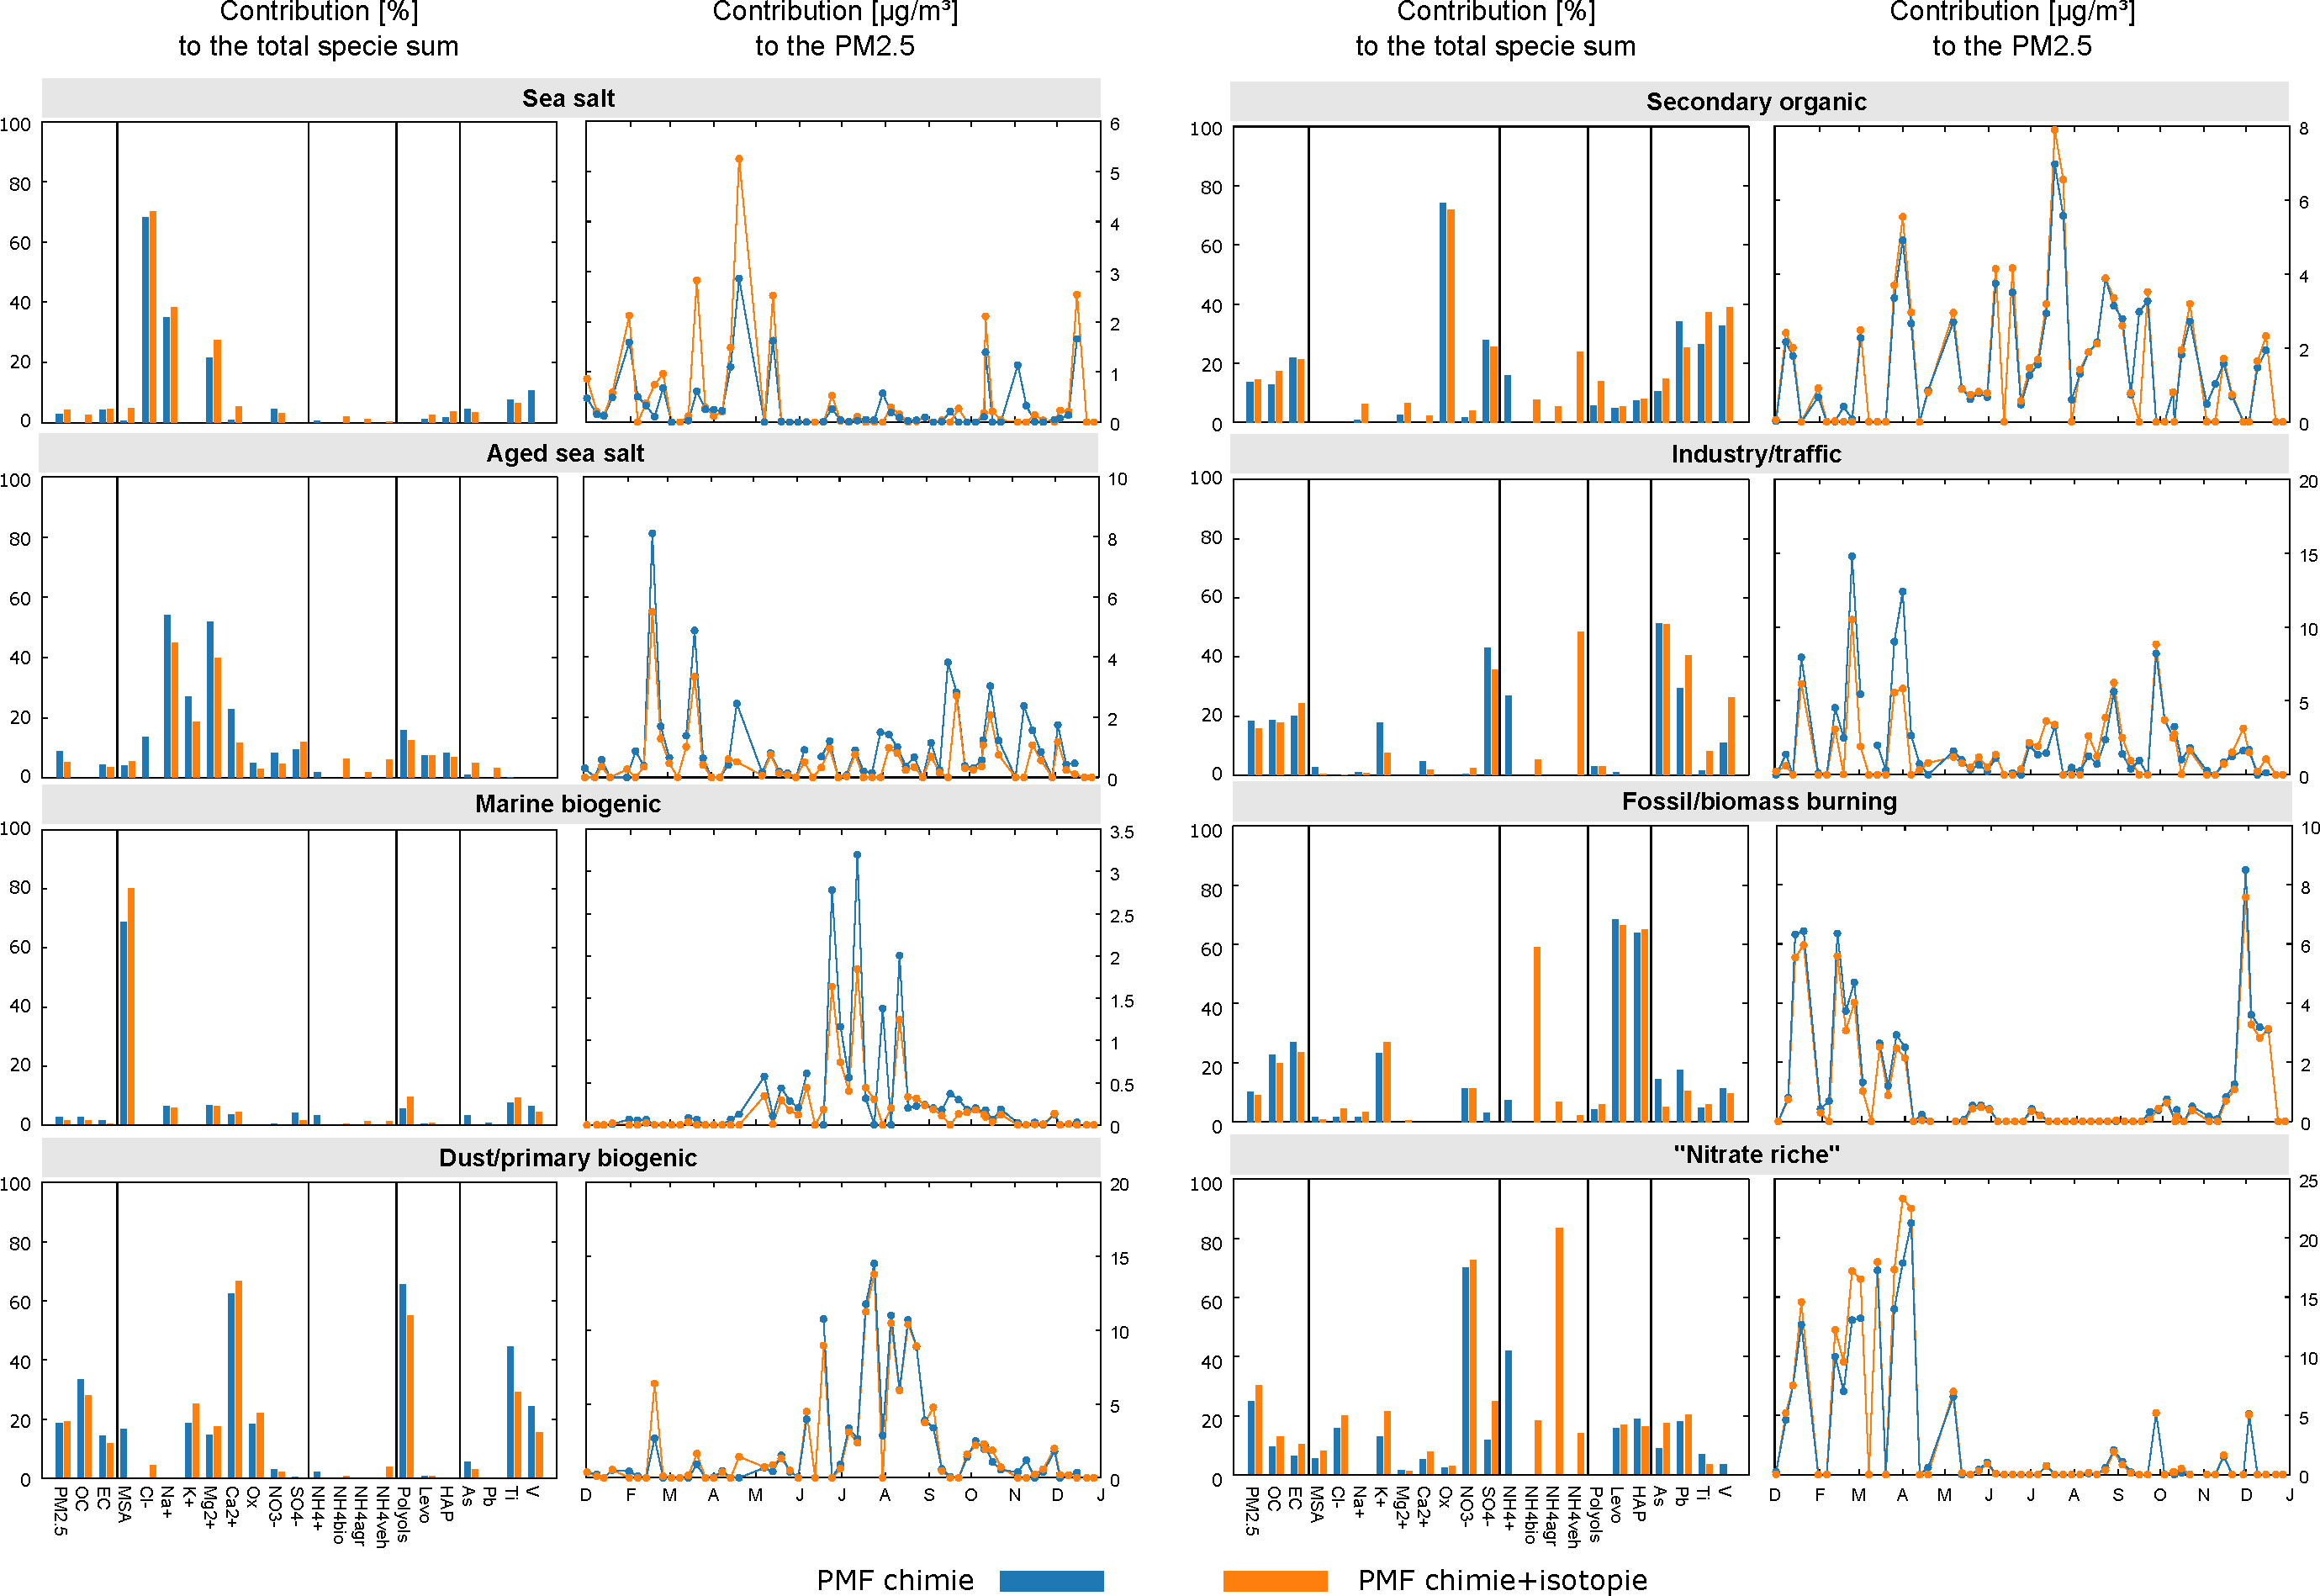
\includegraphics[width=\textwidth]{INACS/PMF_OPE_contrib_profiles.pdf}
    \caption{
        Profils PMF pour une solution à 8 facteurs. Les histogrammes représentent la
        contribution de l'espèce dans chaque facteur par rapport à la masse de l'espèce
        totale et les courbes la contribution temporelle du facteur aux \PMdc{} [\si{\ugm}].
    }
    \label{fig:PMF}
\end{figure}

\paragraph{L'isotopie est-elle respectée ?}%
\label{par:l_isotopie_est_elle_respectée_}

Finalement, il est important de vérifier que la valeur isotopique reconstruite par les
concentrations de \NHq{} estimées par la PMF sont proches des valeurs estimées par méthode
Monte-Carlo.

Si les concentrations estimées par la PMF sont proches du modèle Monte-Carlo en été, on
observe cependant une erreur plus importante durant les pics de pollution (voir
figure~\ref{fig:PMFreconstruct}.a).
La conséquence est une reconstruction de l'isotopie moins bonne pendant ces périodes
(figure~\ref{fig:PMFreconstruct}.c).
Plus important encore, les prédictions de la PMF sont en dehors des écart-types du modèle
Monte-Carlo pour les pics de pollutions de fin février et fin mars-début avril, alors même
que la quantité totale d'ammonium est respectée (figure~\ref{fig:PMFreconstruct}.b).

Il est donc important de noter que les résultats de la PMF couplée vont dans le sens d'une
meilleure attribution des sources mais possèdent néanmoins encore une marge d'évolution
importante.
En \og forçant \fg{} davantage la PMF d'après les données issues de Monte-Carlo,
l'importance du facteur agricole augmenterait et celle du trafic/industrie diminuerait.
L'estimation PMF présentée ici est donc une estimation basse de l'importance du facteur
agricole.

\begin{figure}[ht]
    \centering
    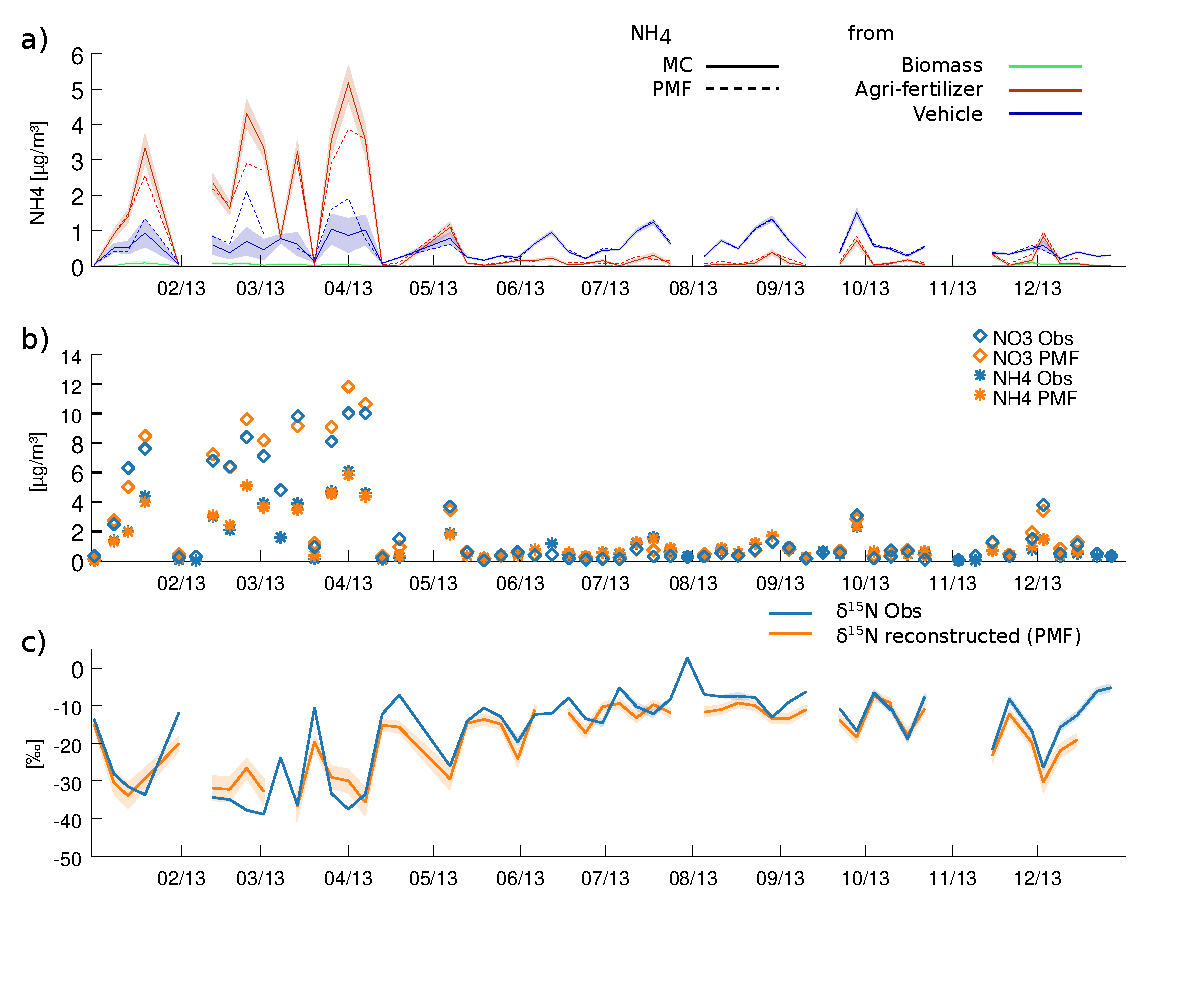
\includegraphics[width=1.0\textwidth]{figures/INACS/PMF_OPE_reconstruction.pdf}
    \caption{Reconstruction des variables \textbf{a)} \NHq$_{src}$, \textbf{b)} \NOt~et
        \NHq$_{tot}$ et \textbf{c)} \dN~par modèle inverse d'après les données de sorties
        de PMF.
        \textbf{b)} Le \NOt~prédit est celui reconstruit par la PMF et le \NHq~est la
        somme des trois \NHq$_{src}$ donnés par la PMF.
        \textbf{c)} L'observation isotopique \dN~est notée en trait plein bleu et le
        \dN~reconstruit depuis les \NHq estimés par PMF en orange dont l'incertitude
        correspond à l'écart type de 2000 tirages aléatoires des valeurs des sources.
    }
    \label{fig:PMFreconstruct}
\end{figure}

\subsubsection{Conclusion}%
\label{ssub:conclusion_isotopie}


Grâce à l'isotopie, nous avons pu montrer que l'ammonium provient très majoritairement
de la source agricole lors des pics de pollutions printanier, et ce à très grande échelle
spatiale, alors que la source véhiculaire constituant le fond ambiant tout le long de
l'année.

Également, la méthodologie établie permet l'utilisation d'informations isotopiques dans
une étude PMF alors même que l'isotopie n'est pas additive, à condition d'effectuer un
traitement préalable du signal isotopique. Une contrainte forte de cette méthode est la
connaissance préalable de la signature isotopique des sources, ce qui rend la PMF moins
``agnostique'' sur la géochimie des facteurs.

Ainsi, la contribution du secteur agricole du facteur ``Nitrate rich'', déterminé dans de
nombreuseis PMF, est maintenant démontrée sur le site de l'OPE.
L'ajout de l'information isotopique permet également d'affiner la contribution et les
profils chimiques des autres facteurs contenant de l'ammonium, les rendant plus proches de
ce que l'on s'attend à observer (contribution du trafic homogène sur l'année, etc).

Cependant, l'une des limitations majeures concerne le choix des sources d'ammonium
considérées. Cette limitation est davantage explorée dans l'annexe~\ref{annexe:INACS}.

\todo{faire une phrase de conclusion}

\subsection{Émission biogénique primaire}%
\label{sub:émission_biogénique_primaire}

\subsubsection{Problématique : la matière organique}%
\label{ssub:problématique_la_matière_organique}

La matière organique présente une large part d'espèce non identifiée et peut avoir de
nombreuse provenances. Bien que pour certaines sources, différentes espèces nous
permettent d'identifier et quantifier la contribution de différentes sources à la matière
organique (lévoglucosan et potatium pour la combustion de biomasse par exemple), certaines
espèces organiques mesurées ne présentent pas de corrélation évidente avec les facteurs PMF
lorsqu'aucun de ceux-ci n'est identifié comme provenant des émissions biogéniques. C'est
notamment le cas de l'arabitol et mannitol, composés émis par les champignons et
bactéries.

Aussi, la microbiologie présente sur les aérosols peut influer de manière importante
sur le PO des aérosols \autocite{samakeUnexpected2017}.

Ainsi, mieux quantifier et identifier la provenance des sources d'émissions biogéniques
primaires permettrait peut-être d'identifier l'une des raisons de la sous-estimation des
PM par les modèles CTM, en pointant une source actuellement mal prise en compte dans ces
modèles.

\begin{tcolorbox}[colback=red!5!white,colframe=Melon,title=Note]
    Cette étude a été menée dans le cadre de la thèse de~\cite{samakeAtmospheric2019}, et
    mon implication dans ces travaux concerne la partie recensement des données à partir
    de la base de donnée établie et présentée
    section~\ref{sec:harmonisation_et_gestion_de_base_de_donnée}, ainsi que l'utilisation
    et le traitement des résultats issues des PMF des projets DECOMBIO et SOURCES
    (présentée en détail section~\ref{sec:sources}).
\end{tcolorbox}

\subsubsection{Synthèse grande échelle de la climatologie des polyols}%
\label{ssub:synthèse_grande_échelle_de_la_climatologie_des_polyols}

Pour comprendre la dynamique spatiale et temporelle des émissions biogéniques primaires,
28 stations française présentant a minima un cycle annuelle de prélèvement analysant
l'arabitol, sorbitol, mannitol et glucose ont été
selectionnées~\autocite{samakePolyols2019}.

Ainsi, nous avons montré que l'arabitol et mannitol présente de très forte corrélation 
($0.58 \leq r^2 \leq 0.93$), avec un coefficient de droite de régression entre 0.59 et
1.10 pour un intercepte faible (toujours inférieur à \SI{9}{\ngm})). Ainsi, il parait
raisonable de penser que ces 2 espèces sont co-émisent par une ou plusieurs sources.
Le sorbitol et le glucose présentent quant à eux des dynamiques propres, non nécessairement corrélés à ces
deux espèces.
L'arabitol et le mannitol sont sommées et appelé \textit{polyols} par la suite.

Les polyols, en plus d'être ubiquitaire, présente le même signal saisonnier sur l'ensemble
des sites d'études (voir figure~\ref{fig:polyols_samake2019}) et sont davantage présent
dans la fraction grossière (\PMdix) que fine (\PMdc), avec des concentrations variant de 
\SI{7.5\pm10.9}{\ngm} à \SI{27.8\pm33.3}{\ngm} pour les \PMdc, et
\SI{48.9\pm38.2}{\ngm} à \SI{73.5\pm61.8}{\ngm} pour les \PMdix, sur respectivement le site de
Revin et de l'OPE, correspondant à un ratio \PMdix/\PMdc{} variant en moyenne de 3 à 5.
Cette ségrégation suivant la taille des particules est identique pour le glucose.

Les polyols ne représentent cependant qu'une faible fraction de la matière organique. En effet, en
considérant un ratio entre l'OM et l'OC de 1.8 typique des écosystèmes d'Europe de
l'ouest, les polyols ne représentent qu'entre 0.1 et 2.1\%. La même contribution relative
est trouvée pour le glucose.

\begin{figure}[ht]
    \centering
    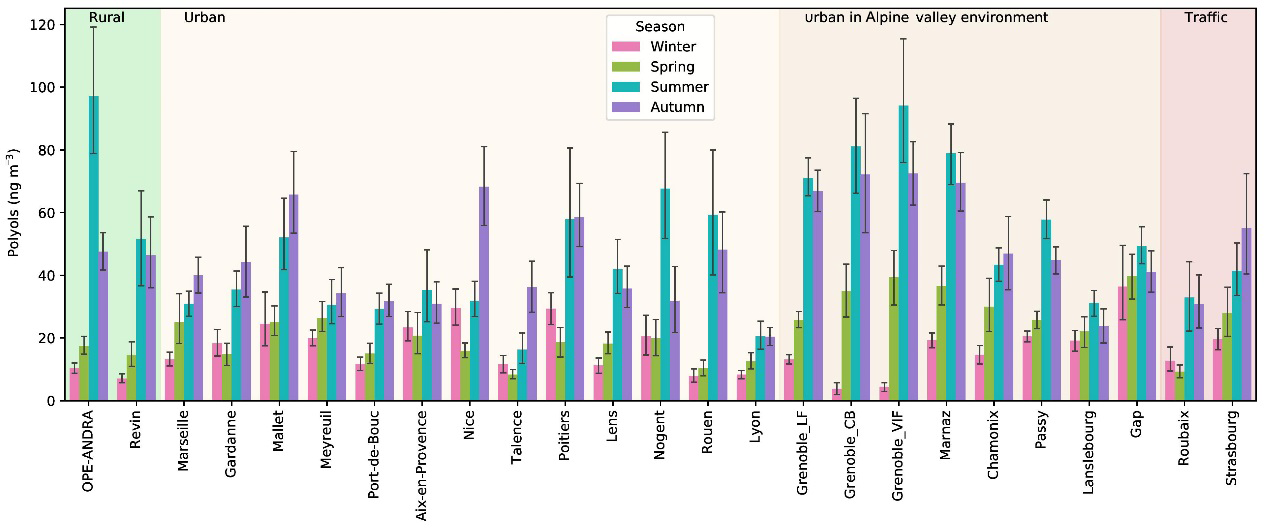
\includegraphics[width=1\linewidth]{chapter03/polyols_samake2019.png}
    \caption{
        Distribution spatio-temporelle des concentrations de polyols (moyenne et écart
        type) en \si{ngm}.
        Source : \cite[figure 6]{samakePolyols2019}.
    }%
    \label{fig:polyols_samake2019}
\end{figure}

La taille des spores ou enveloppes microbiennes, riche en polyols, sont de taille supra
micrométrique (typiquement de \SI{2}{\micro\m} à \SI{10}{\micro\m}), ainsi que l'activité
biologique importante en été et très ralentie en hiver vient grandement conforter
l'hypothèse biogénique de ces composés.

Cette hypothèse a été testée plus en avant par \cite{samakeArabitol2019} sur le site de
l'OPE, où la cellulose a été mesurée sur 2 années de prélèvements, ainsi que
l'enregistrement des différentes activités agricoles avoisinantes (voir
figure~\ref{fig:ope_polyols_cellullose_agri}).
La coïncidence entre l'augmentation des polyols, de la cellulose (traceuse des débris de
plante) et des moissons mais beaucoup moins des labours conforte encore une fois la provenance
biogénique, mais précise cette fois le compartiment en question : les polyols proviennent
très certainement des plantes et non du sol.

Pour s'en assurer, une troisième étude, analysant l'ADN de prélèvement d'échantillon
de plantes, de sols et d'aérosols du site l'OPE, \autocite{samakeHigh2020} précise que
l'ADN retrouver dans les aérosols correspond bien des taxons de bactéries et champignons
originaires de la strate herbacée et non du sol.

\begin{figure}[ht]
    \centering
    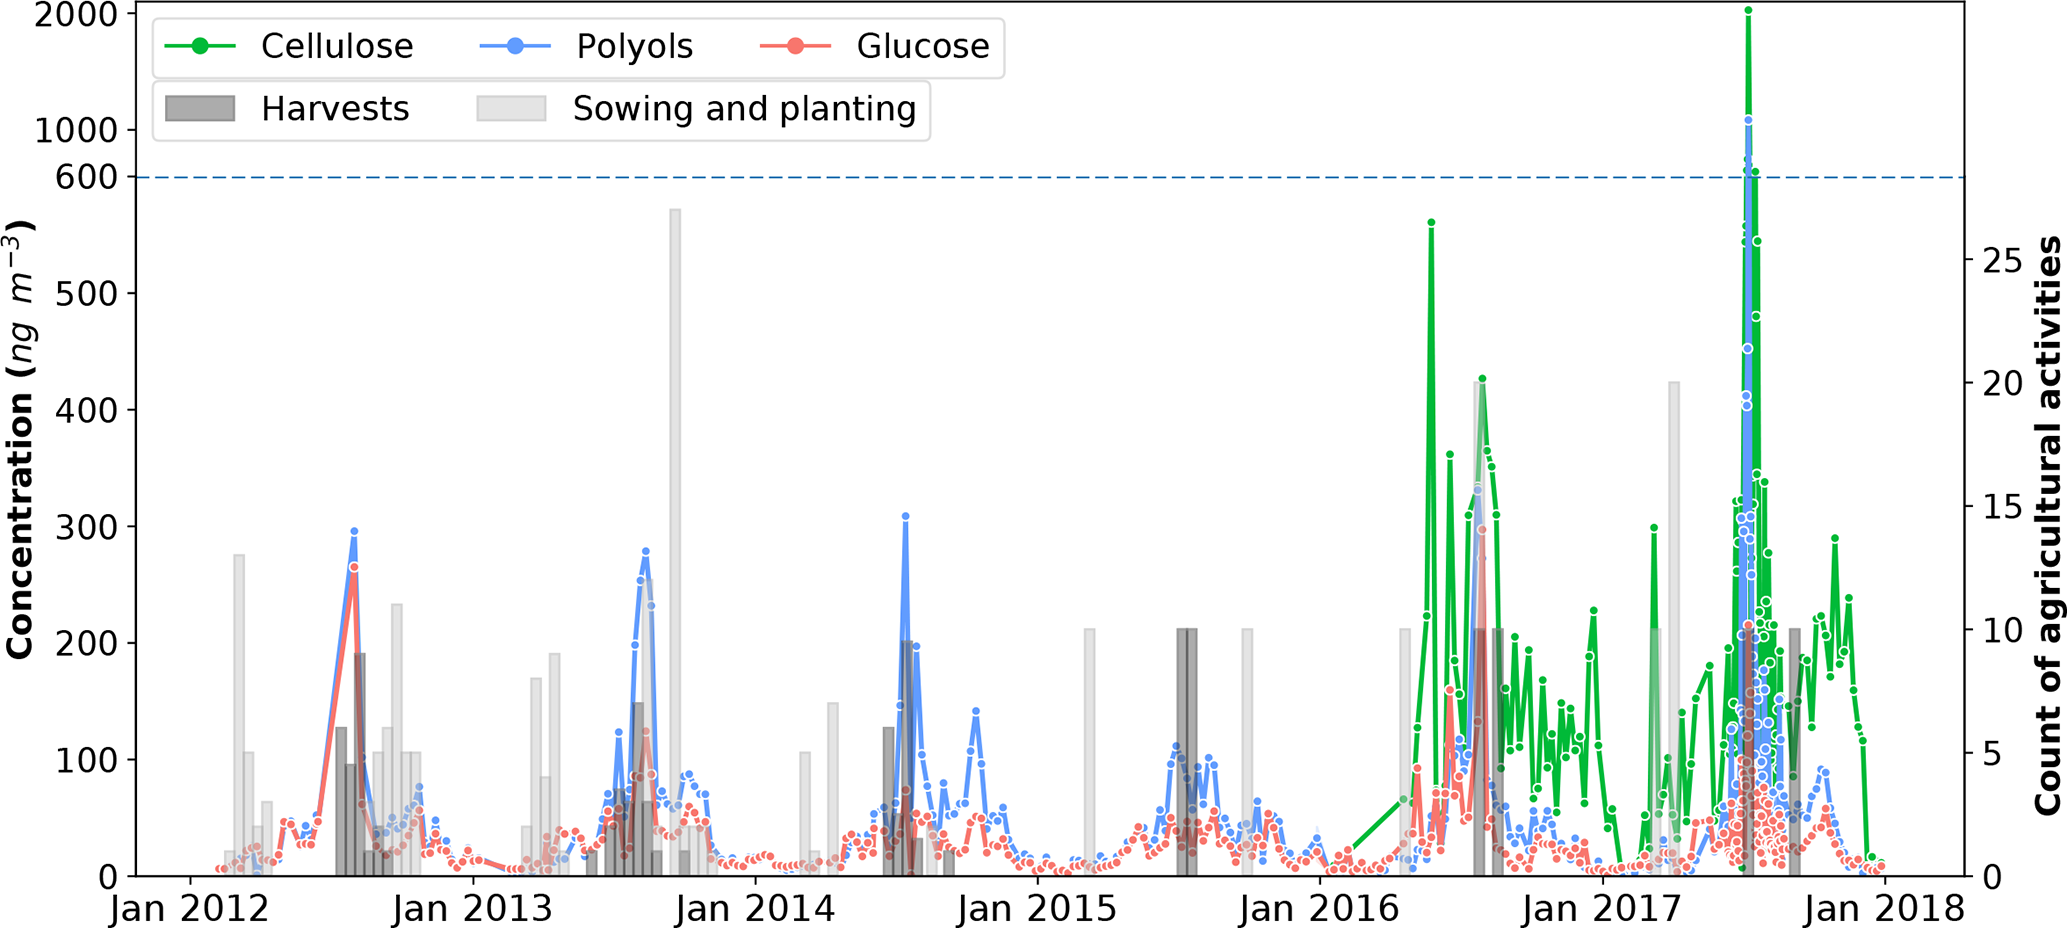
\includegraphics[width=1.0\linewidth]{chapter03/ope_polyols_cellulose_agri_samake2019.png}
    \caption{
        Évolution conjointe des concentrations de polyols, cellulose, glucose et des
        activités agricoles sur le site de l'OPE de 2012 à 2018.
        Les activités de 69 parcelles environnants le site de prélèvement sont
        comptabilisées et agrégées en période de 12 jours.
        Après 2014, seuls les enregistrements pour 2 parcelles étaient disponibles, les
        valeurs sont donc multipliées arbitrairement par 10 pour cette période.
        Source : \cite[figure 6]{samakeArabitol2019}.
    }%
    \label{fig:ope_polyols_cellullose_agri}
\end{figure}

\subsubsection{Contribution des émissions biogéniques primaires aux \PMdix}%
\label{ssub:contribution_des_émissions_biogéniques_primaires_aux_pmdix}

Maintenant que l'origine biogénique des polyols est acquise, il reste à quantifier
l'importance de la source biogénique primaire à l'ensemble des PM.
Puisque les polyols tracent de manière non équivoque cette source, l'ajout de ces espèces dans
les PMF permet d'identifier un profil biogénique primaire.

Pour ce faire, les 16 PMF issues du programme DECOMBIO et SOURCES ont utilisées les polyols
dans le jeu d'espèces sélectionné. Sur ces PMF, un facteur \textit{Primary biogenic
organic aerosol} ou PBOA a systématiquement été identifié, comprenant la quasi-totalité
des polyols.

La contribution de ce facteur à la matière organique totale varie de 6\% à 28\%, pour une
moyenne et écart-type de \SI{13\pm6}{\percent} en moyenne annuelle, mais peut représenter
plus de 40\% de la matière organique en été à certains sites (voir
figure~\ref{fig:chapter03/pboa_pmf_samake2019}).
De fait, cette source d'émission représente un secteur d'émission important pour comprendre
les concentrations ambiantes de PM, notamment en période chaude.

On peut se demander si ce facteur est entièrement d'origine primaire et
n'agrège pas une partie d'aérosol organique biogénique secondaire. En l'absence d'espèce
tracant les processus secondaires (comme le 3-MBTCA ou l'acide pinic), cette possibilité
reste ouverte.
Cette hypothèse parait cependant peu probable. En effet, le ratio OC/polyols du profil
PBOA est relativement peu variable entre les sites, alors qu'il serait peu probable que la
variabilité des processus secondaires conduisent à une concentration d'OC identique sur
l'ensemble des sites.
Aussi, les ratios OC/polyols des profils PBOA (autour de 16) sont bien dans la gamme
attendue de variabilité des spores de champignons (entre 12 et 27), d'après
\cite{bauerSignificant2008,yttriSource2011}.


\todo{expliquer plus en détail la constitution chimique du PBOA ?}

\begin{figure}[ht]
    \centering
    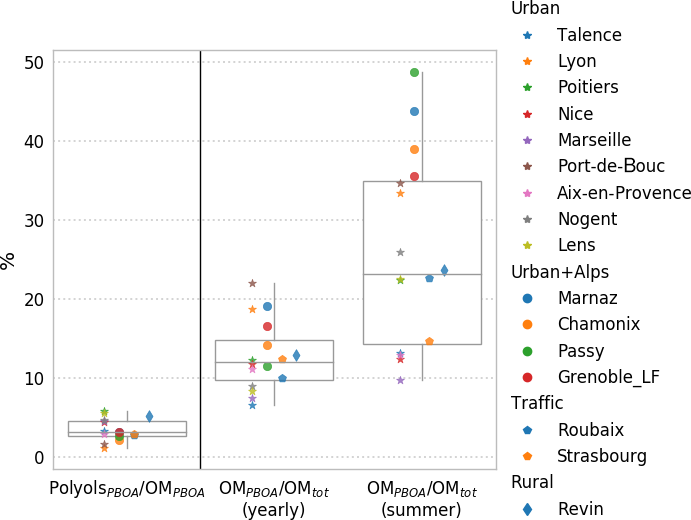
\includegraphics[width=0.7\linewidth]{chapter03/pboa_pmf_samake2019.png}
    \caption{
        Mass contribution of polyols to OM in the PBOA factor, and relative contributions
        of the OM PBOA factor to the total OM in PM for the 16 studied sites where the PMF
        model was run, over the year and summertime only. Stars and circles refer to urban
        sites without and with Alpine valley influence, respectively. Pentagons correspond
        to traffic sites and diamonds to rural sites.
        Source : \cite[figure 9]{samakePolyols2019}.
    }%
    \label{fig:chapter03/pboa_pmf_samake2019}
\end{figure}

\subsubsection{Conclusion}%
\label{ssub:conclusion_polyols}

Nous avons donc montré que les polyols (arabitol et mannitol) sont des traceurs de
l'activité biologiques, notamment de la strate herbacée. Leur présence est ubiquitaire
mais représente seulement 0.1 à 2.1\% de la matière organique.

Ainsi, ces études approfondies sur la dynamique et la provenance des polyols nous ont
permis de les identifier comme étant des espèces traceuses de source unique et présente
sur une large étendue spatiale. Leur ajout dans les études PMF nous permettent donc
l'isolement d'une source biogénique primaire provenant de l'activité biologique fongique
et bactérienne.

Leur ajout dans les analyses multifactorielles nous apprend que la contribution de ce
facteur PBOA à la matière organique totale varie de façons importante selon la saison,
mais peut représenter jusqu'à 40\% de la matière organique en période chaude sur certains
sites étudiés, en faisant un facteur important pour comprendre la dynamique des PM en
période chaude.

Cependant, les polyols ne sont pas la seule source d'émission primaire biogénique (on peut
notamment penser aux débris végétaux par exemple). Aussi, la question de la part
secondaire provenant d'oxydation des composés biogéniques présents dans ce facteur reste
ouverte, en l'absence d'espèce traceuse de processus secondaire comme le 3-MBTCA
ou l'acide pinique. La section suivante~\ref{sub:processus_secondaires} permettra de
répondre en partie à cette question.

\subsection{Variabilité fine échelle, processus secondaires et traceurs organiques}%
\label{sub:processus_secondaires}

Afin de tenter de répondre à la problématique de la contribution des facteurs secondaires
aux PM, 3 sites de prélèvement sur Grenoble et périphérie (fond urbain : Les frènes (LF),
hypercentre : Caserne de bonne (CB) et périurbain : Vif (Vif)) ont été choisi pour établir une
étude PMF incluant de nouveaux traceurs organiques spécifiques des processus d'oxydations
secondaires : le 3-MBTCA, l'acide pinique et phtalique. Sur cette étude, la cellulose a
également été mesurée pour essayer de distinguer potentiellement différentes émissions
biogéniques.

Aussi, la proximité géographique des 3 sites --tous dans un rayon de \SI{15}{\kilo\m}--
permet l'estimation de la variabilité fine échelle de l'ensemble des sources identifiées
par la PMF.

\begin{tcolorbox}[colback=red!5!white,colframe=Melon,title=Note]
    Cette partie s'appuie sur les travaux de \cite{borlazaFinescaleinprep.}, dont je suis
    second auteur, lors du projet Mobil'Air, destiné également à évaluer l'impacte sur la
    qualité de l'air d'une zone à faible émission dans la métropole grenobloise 
    (\url{https://mobilair.univ-grenoble-alpes.fr/}).
\end{tcolorbox}

\subsubsection{Variabilités saisonières}%
\label{ssub:variabilites_saisonières}

La cellulose étant très peu couramment mesuré, ainsi que les acides organiques, est içi
présenté dans un premier temps les mesures de concentrations obtenues sur l'année
2017-2018 pour les 3 sites, en comparaison avec d'autres espèces plus communément mesurées.

\paragraph{Corrélation entre espèces}%
\label{par:correlation_entre_especes}

\subparagraph{Oxydation secondaire biogénique}%
\label{par:oxydation_secondaire_biogénique}

On s'aperçoit tout d'abord que le 3-MBTCA et l'acide pinique présentent de très forte
corrélation sur les 3 sites, avec un cycle saisonnier fort et de forte concentration en été
(voir figure~\ref{fig:borlaza_evolution_temporelle}). Du fait de l'activité photochimique
conduisant à la formation d'espèce secondaire issue des terpènes en cette période, ce
résultat était attendu. On observe aussi de forte variation de concentration à faible
échelle temporelle (de l'ordre de quelques jours). Ces espèces sont en effet très réactive
et présente un temps de demie-vie très courte dans l'atmosphère.

Aussi, ces espèces partagent le cycle saisonnier du MSA, mais présentent cependant des
contributions asynchrones, indiquant alors différents processus secondaires.

\subparagraph{Polyols et cellulose}%
\label{par:oxydation_secondaire_anthrophique}

Comme attendue d'après \cite{samakePolyols2019}, les polyols ont un cycle saisonier très
marqués avec une forte concentration en été et faible en hiver. Ce cycle est aussi présent
pour la cellulose, bien que moins marqué cependant. En revanche, la durée où de la
cellulose est présente dans l'atmosphère est beaucoup plus grande que pour les polyols.
Ainsi, les sources émettrices de polyols et de cellulose ne peuvent pas être entièrement
les mêmes.

\subparagraph{Sulfate et acide phthalic}%
\label{par:sulfate_et_acide_phthalic}

L'acide phthalique est en très faible concentration tout le long de l'année d'étude,
exceptés quelques pics très restreints temporellement. La synchronicité de ces pics avec de
forte concentration en sulfate est également observée, mais n'est pas bien comprise pour
l'instant.


\begin{figure}[ht]
    \centering
    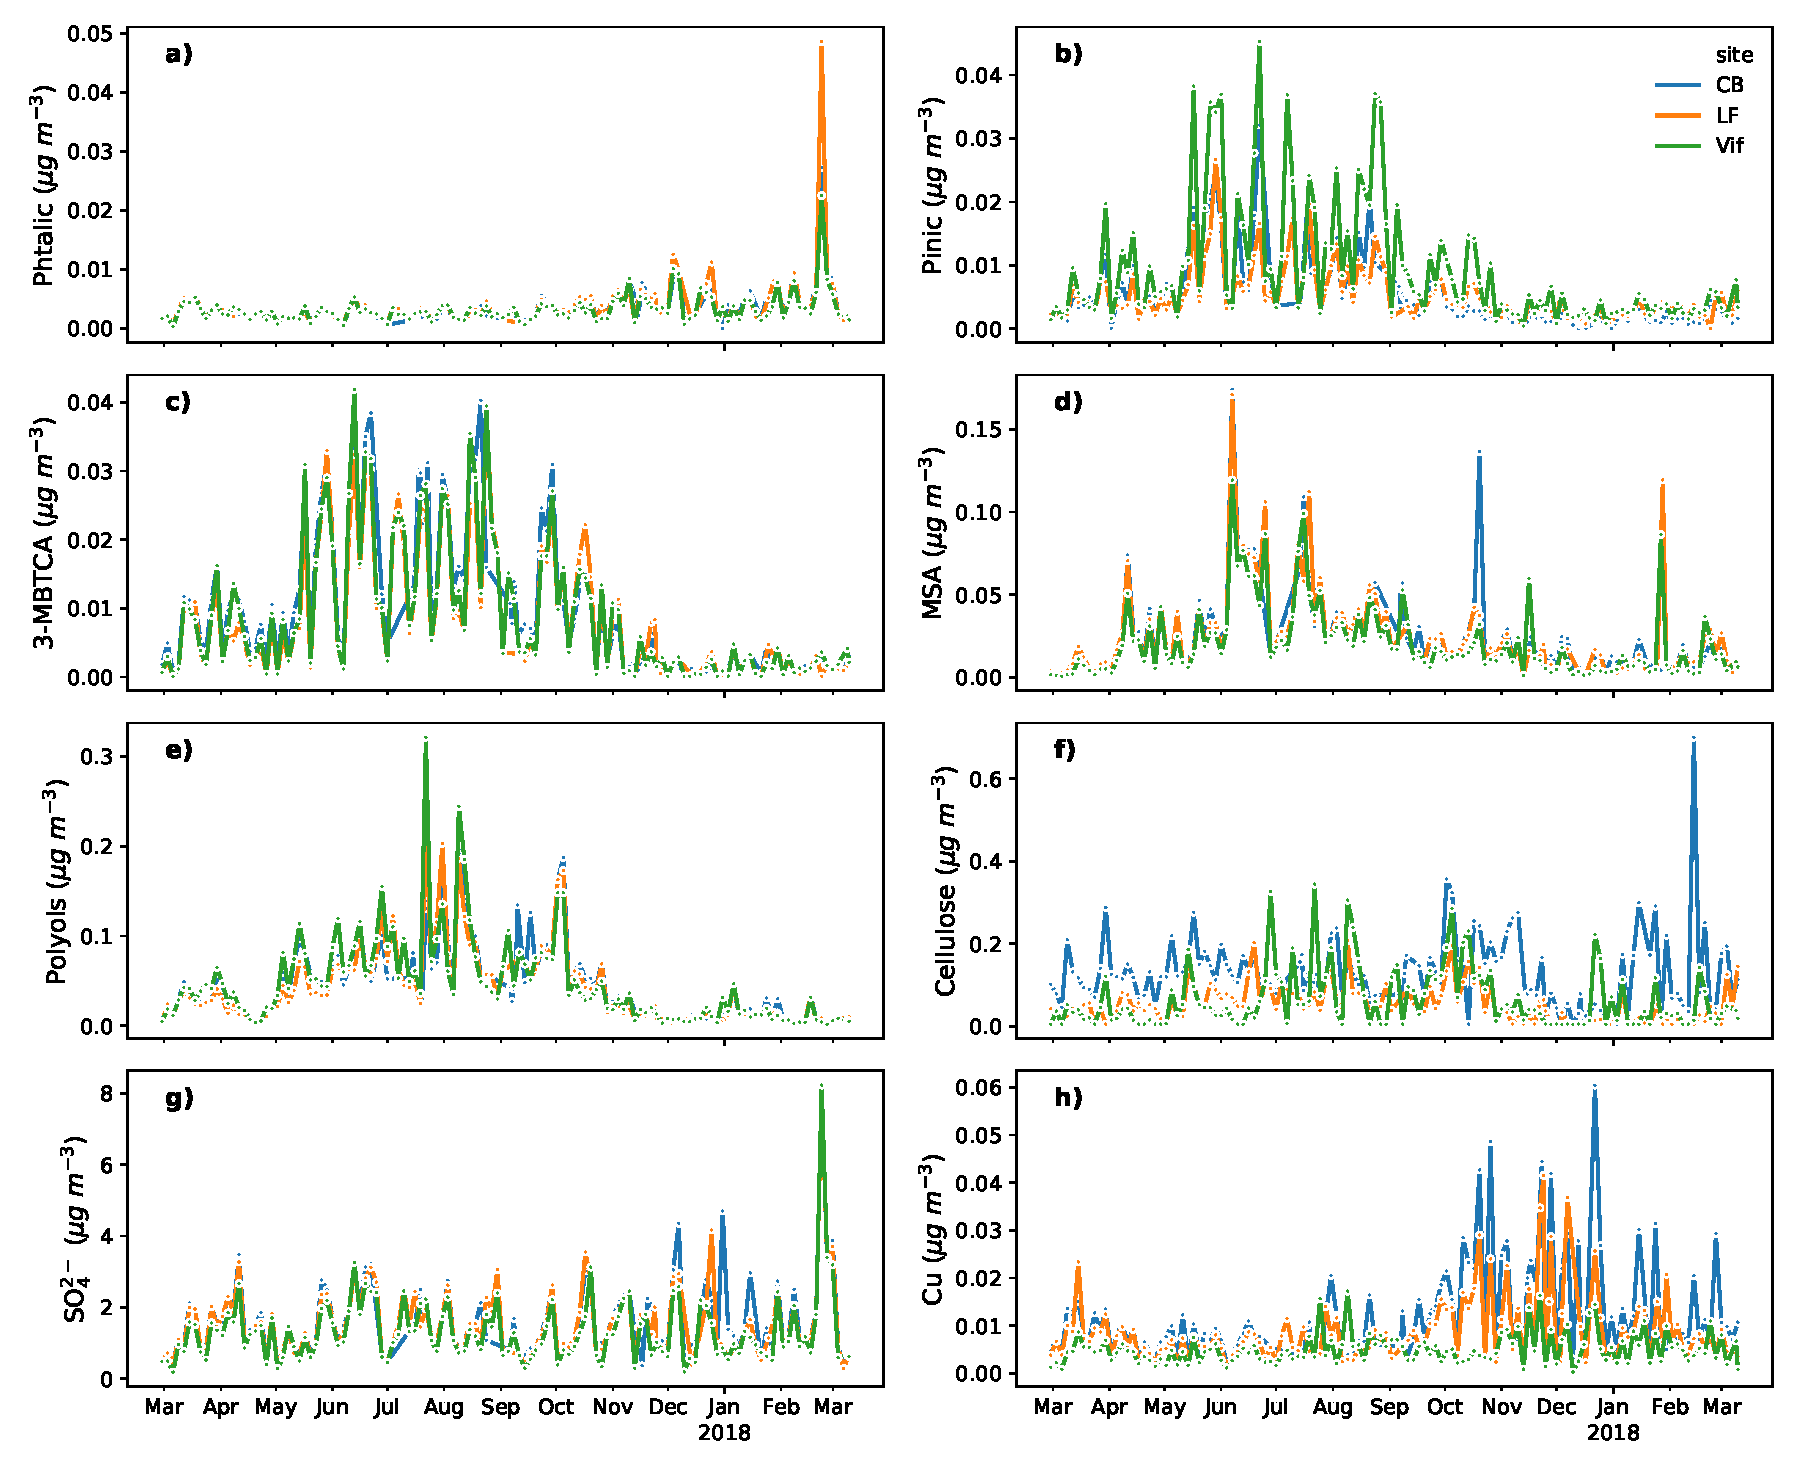
\includegraphics[width=1\linewidth]{chapter03/borlaza/AllInOne.pdf}
    \caption{
        Évolution temporelle de \textbf{a)} l'acide phthalic, \textbf{b)} l'acide pinic,
        \textbf{c)} le 3-MBTCA, \textbf{d)} le MSA, \textbf{e)} les polyols
        (arabitol+mannitol), \textbf{f)} la cellulose, \textbf{g)} le sulfate et
        \textbf{h)} le cuivre pour les 3 sites du bassin grenoblois (LF en orange, CB en
        bleu et Vif en vert).
    }%
    \label{fig:borlaza_evolution_temporelle}
\end{figure}

\paragraph{Similitude et diversité inter-site}%
\label{par:similitude_et_diversité_inter_site}

Lorsque l'on compare les sites entre eux
(figure~\ref{fig:chapter03/borlaza/correlation}), de très fortes corrélations sont
observées pour les ions et espèces organiques, à l'exception notoire de la cellulose, qui
semble avoir une dynamique propre sur chacun des sites.

Les traceurs du trafic routier (Cu et Fe) semble indiquer une proximité entre les sites de
LF et CB, alors que le site de Vif présente un signal différent. Il en est de même pour
les traceurs des poussières crustales (\ce{Ca^{2+}}, Al et Ti). Bien que la distance entre
le centre de Grenoble et le site de Vif puisse expliquer cette différence, il n'est pas à
exclure que la présence d'un terrain de cross à proximité de la station de Vif rende ces
mesures singulières et non représentatives d'un fond périurbain.

\begin{figure}[ht]
    \centering
    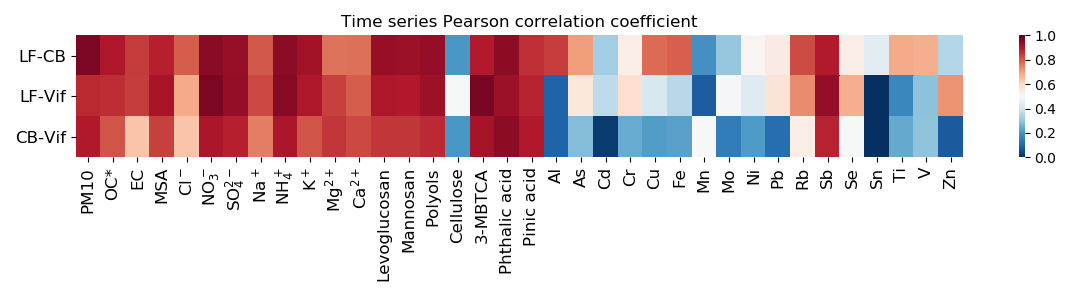
\includegraphics[width=1\linewidth]{chapter03/borlaza/correlation.png}
    \caption{Corrélation de pearson des concentrations temporelle des espèces mesurée
    entre les 3 pairs de site (LF-CB, LF-Vif et CB-Vif)}%
    \label{fig:chapter03/borlaza/correlation}
\end{figure}

\subsubsection{Résultats PMF}%
\label{ssub:résultats_pmf}

Afin d'estimer l'impacte de l'ajout de la cellulose, acide pinique et phthalique et 3-MBTCA,
une PMF ``classique'' (i.e. sans ces nouvelles espèces) sert de référence, et une PMF
``organique'' incluant ces espèces mais respectant strictement les autres paramètres de la
PMF classique permet l'évaluation de leurs effets.
Les PMF sont calculées indépendamment pour les 3 sites.
10 facteurs sont identifiés sur les 3 sites pour la PMF classique, résumés dans le
tableau~\ref{tab:pmf_mobilair_species}.

\begin{table}[ht]
    \begin{ThreePartTable}
        \centering
        \caption{Résumé des facteurs PMF identifiés sur les 3 sites grâce à leurs traceurs
        spécifiques.}
        \footnotesize
        \label{tab:pmf_mobilair_species}
        \begin{tabular}{ll}
            \toprule
            Identified factors & Specific tracers\\
            \midrule
            Biomass burning              & Levoglucosan, mannosan, \ce{K+}, Rb, \ce{Cl-}\\
            Primary traffic              & EC, \ce{Ca^{2+}}, Cu, Fe, Sb, Sn\\
            Nitrate-rich                 & \ce{NO3-}, \ce{NH4+}, phthalic acid\\
            Sulfate-rich                 & \ce{SO4^{2-}}, \ce{NH4+}, Se, phthalic acid \\
            Mineral dust                 & \ce{Ca^{2+}}\tnote{*}, Al, Ti, V\\
            Sea/road salt                & \ce{Na+}, \ce{Cl-}\\
            Aged sea salt                & \ce{Na+}, \ce{Mg^{2+}} \\
            Industrial                   & As, Cd, Cr, Mn, Mo, Ni, Pb, Zn\\
            Primary biogenic             & Polyols, cellulose\\
            MSA-rich                     & MSA\\
            Secondary biogenic oxidation\tnote{a} & 3-MBTCA, pinic acid\\
            \bottomrule
        \end{tabular}
        \begin{tablenotes}
        \item[*] Le site de Vif ne présente pas \ce{Ca^{2+}} dans ce facteur.
        \item[a] Seulement identifié pour les PMF organiques.
        \end{tablenotes}
    \end{ThreePartTable}
\end{table}

\paragraph{Nouveau facteur d'oxydation secondaire biogénique}%
\label{par:nouveau_facteur_d_oxydation_secondaire_biogénique}

Lors de l'ajout des nouvelles espèces organiques, un nouveau facteur apparaît, riche en
3-MBTCA et acide pinique et dont la contribution est maximale en été (voir la composition
et contribution temporelle de ce profil sur le site de CB
figure~\ref{fig:chapter03/borlaza/CB-SBO}).
Ce facteur apporte jusqu'à \SI{10}{\ugm} de \PMdix{} certains jours d'été, en faisant l'un
des facteurs majeurs contribuant aux \PMdix{} certains jours.
Aussi, une part importante de l'OC est amené par ce facteur (environ 10\% de l'OC
total), mais également du sulfate (environ 15\%), suggérant la présence de composés
organiques suflatés.
Ainsi, en moyenne estivale, c'est entre 20\% et 40\% de la matière organique qui est
apporté par ce facteur selon le site considéré, ce qui en fait le facteur principal
d'apport de matière organique pendant cette période.

\paragraph{Primaire biogénique}%
\label{par:primaire_biogénique}

Le deuxième facteur présentant d'importante contribution de ces traceurs organiques est
le profile d'émission primaire biogénique (voir
figure~\ref{fig:chapter03/borlaza/LF-PBOA}). Notamment, près de 60\% de la cellulose est
apporté par ce facteur, renforcant l'hypothèse de l'émission de ce facteur par la strate
herbacée (comme expliqué en section~\ref{sub:émission_biogénique_primaire}). Aussi, et
comme suspecté auparavant, ce facteur est également responsable d'environ 20\% de l'acide
pinique et du 3-MBTCA, et par conséquent une part de la matière organique n'est pas
d'origine primaire mais secondaire, bien que limité. Il est à noter également que la
quantité totale de matière organique ou de \PMdix{} expliqué par ce facteur ne varie
pas avec l'ajout de ces nouveaux traceurs organiques (voir
figure~\ref{fig:chapter03/borlaza/comparaison-classique-orga}), et de manière générale, à
part l'ajout de la cellulose et de l'acide pinique et 3-MBTCA, la
composition chimique de ce facteur reste identique entre la PMF de référence et la PMF
organique.

\begin{figure}[ht]
    \centering
    \begin{subfigure}[t]{1\textwidth}
    \begin{center}
        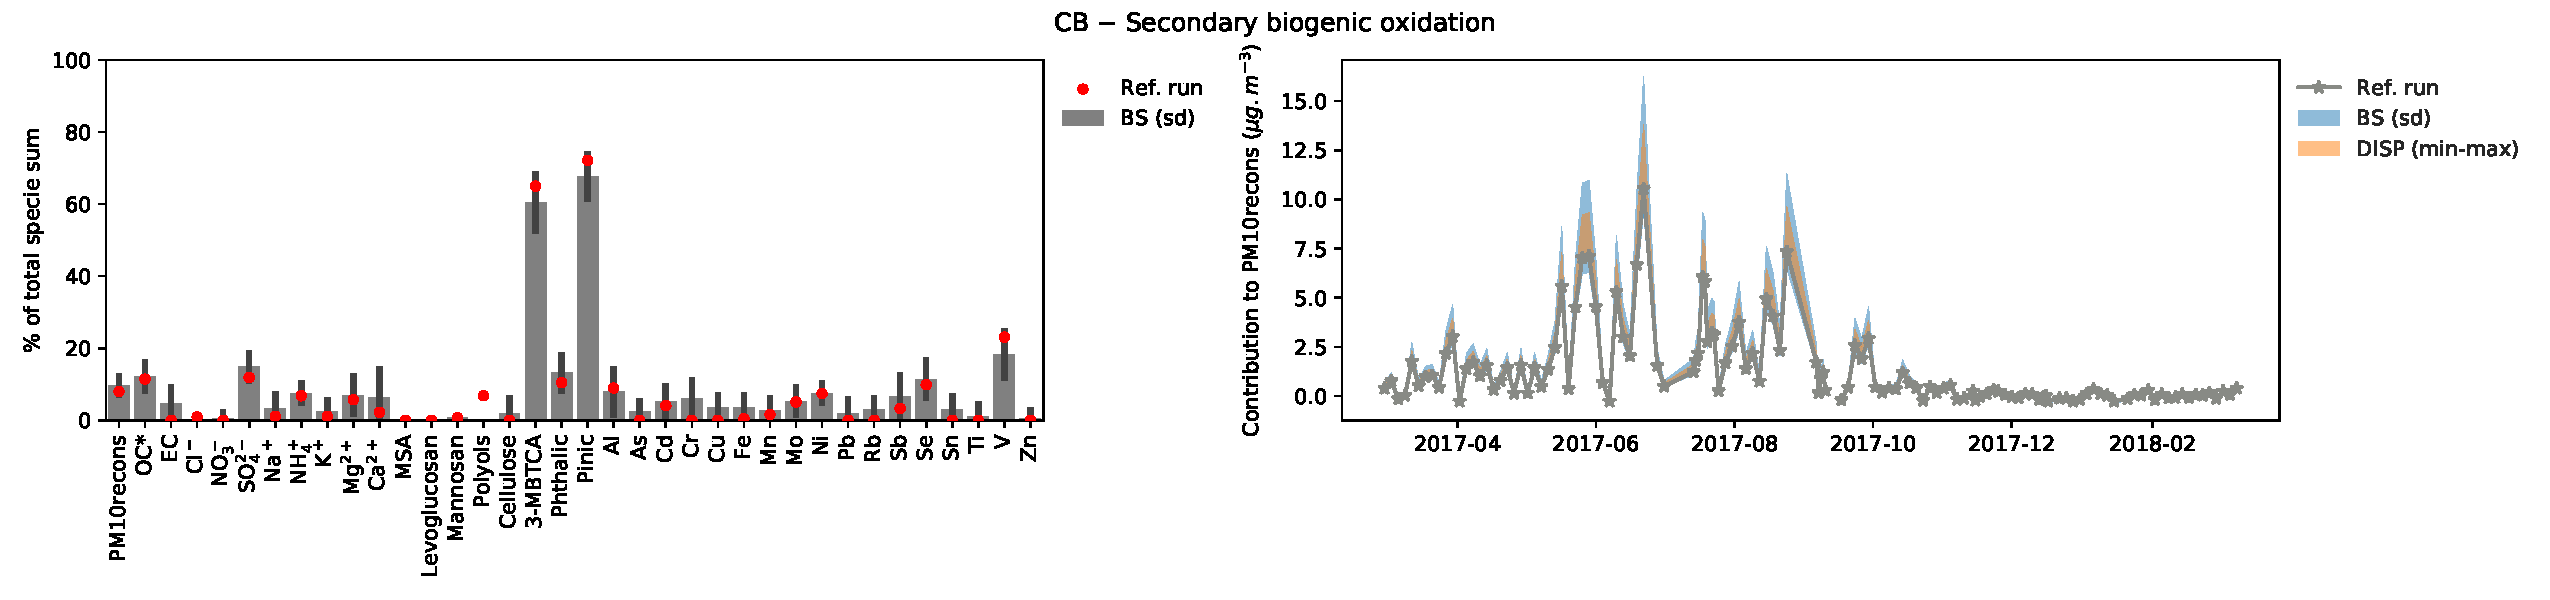
\includegraphics[width=1\linewidth]{chapter03/borlaza/CB-Secondary biogenic oxidation.pdf}
    \end{center}
    \caption{Composition chimique et contribution temporelle aux \PMdix{} du facteur
    d'oxydation biogénique secondaire sur le site d'hypercentre CB.}%
    \label{fig:chapter03/borlaza/CB-SBO}
    \end{subfigure}
    \begin{subfigure}[t]{1\textwidth}
    \begin{center}
        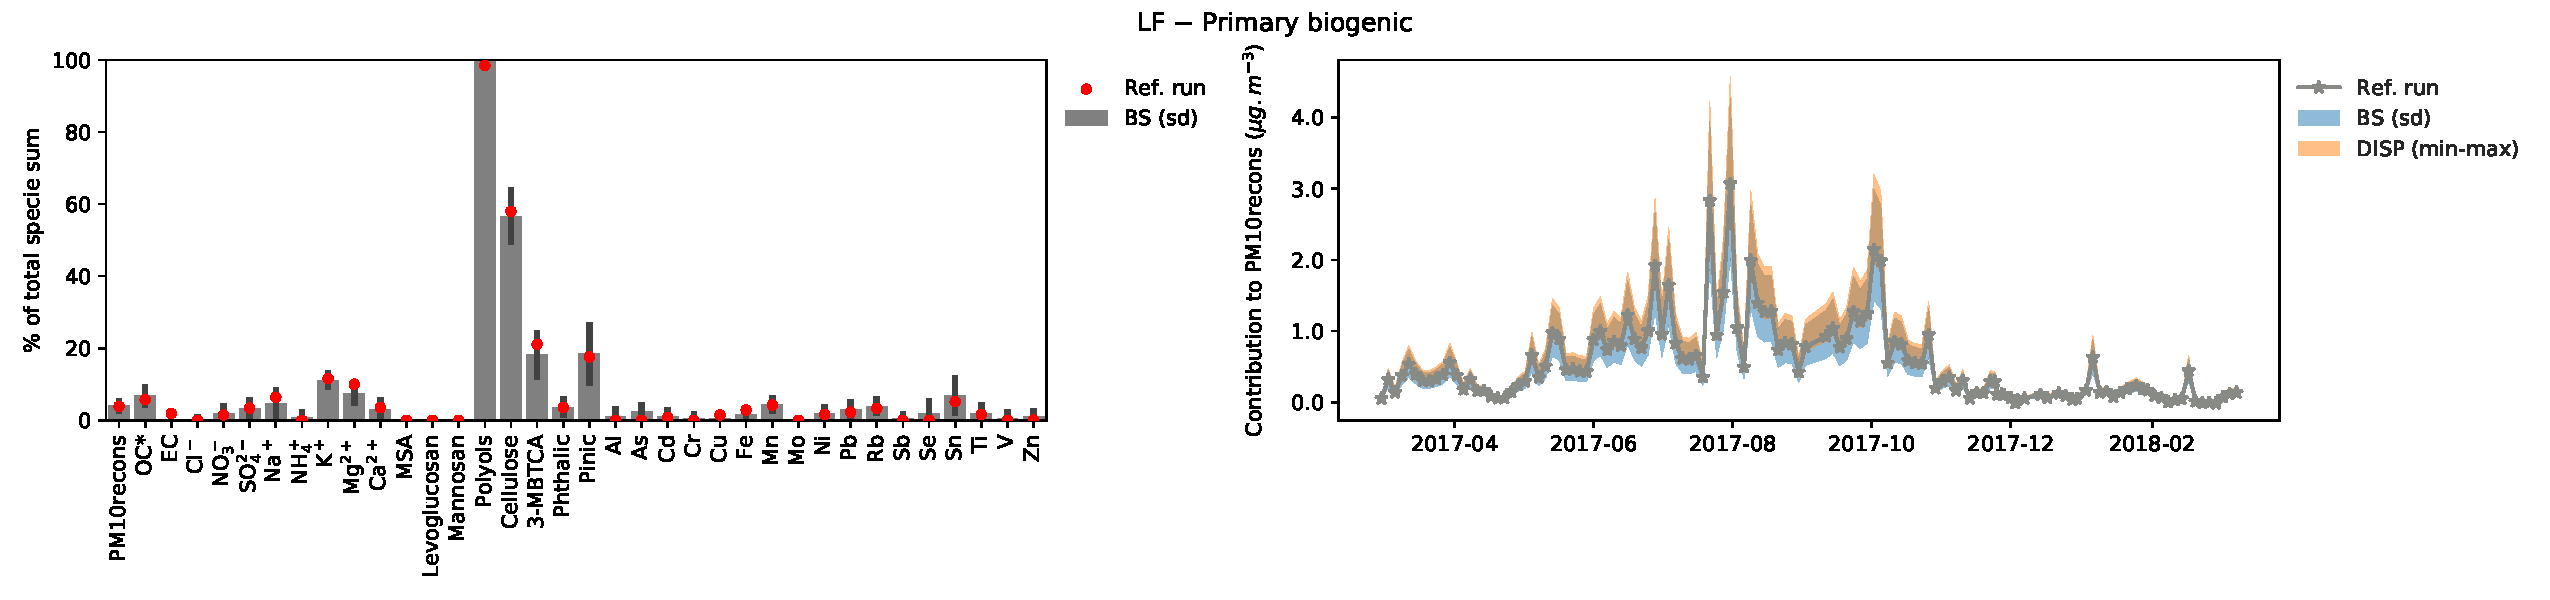
\includegraphics[width=1\linewidth]{chapter03/borlaza/LF-Primary biogenic.pdf}
    \end{center}
    \caption{Composition chimique et contribution temporelle aux \PMdix{} du facteur
    d'émission primaire biogénique sur le site de fond urbain LF.}%
    \label{fig:chapter03/borlaza/LF-PBOA}
    \end{subfigure}
    \caption{Profile chimique et contribution temporelle aux \PMdix{} des 2 facteurs
        majoritairement impactés par l'ajout de la cellulose, acide pinique et phthalique
        et 3-MBTCA.
    }%
    \label{fig:chapter03/borlaza/pmf_profiles}
\end{figure}

\begin{figure}[ht]
    \centering
    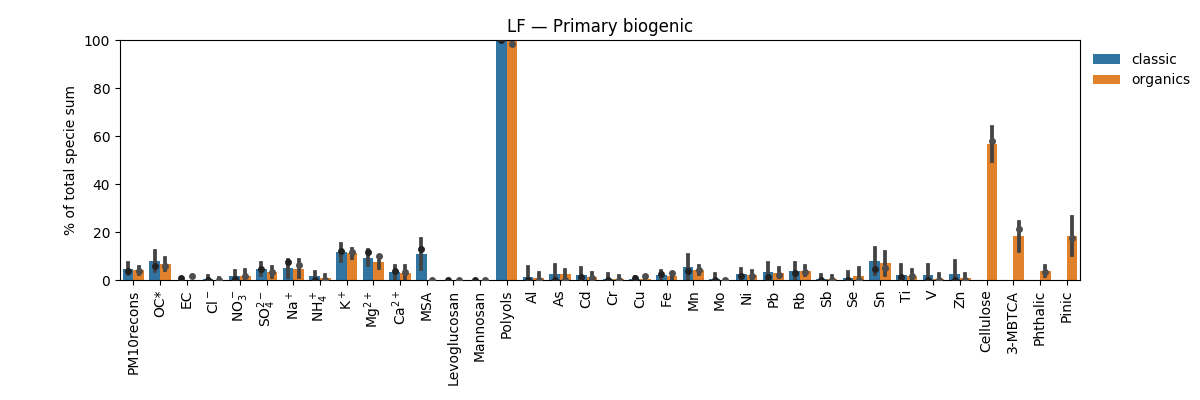
\includegraphics[width=1\linewidth]{chapter03/borlaza/Comparison_orga-woOrga_profile_Primary biogenic_LF.png}
    \caption{Comparaison du profil chimique du facteur primaire biogénique sur le site de
        fond urbain LF entre la PMF classique (en bleue) et celle incluant les nouvelles
    espèces organiques (en orange).}%
    \label{fig:chapter03/borlaza/comparaison-classique-orga}
\end{figure}

\paragraph{Contributions des facteurs aux \PMdix}%
\label{par:contributions_des_facteurs_aux_pmdix}

Comparés aux PMF classiques, la différence majeure de la contribution aux \PMdix{} réside en
la diminution de l'importance du facteur sulfate rich au profit de l'oxydation biogénique
secondaire (voir figure~\ref{fig:chapter03/borlaza/Comparison_orga-woOrga_absolute}).
En effet, on observe une baisse entre \SI{1}{\ugm} et \SI{2}{\ugm} de la contribution du
facteur sulfate rich en moyenne annuelle sur les 3 sites, et une contribution équivalente à
la baisse du suflate rich pour le nouveau facteur d'oxydation secondaire biogénique.

Ainsi, l'ajout des nouveaux traceurs organiques a permis de mieux séparer le facteur
sulfate rich, qui comportait une part importante de l'OC, en deux facteurs de typologie
plus claire : secondaire inorganique sulfaté (i.e. sulfate rich) et secondaire organique
biogénique.

\begin{figure}[ht]
    \centering
    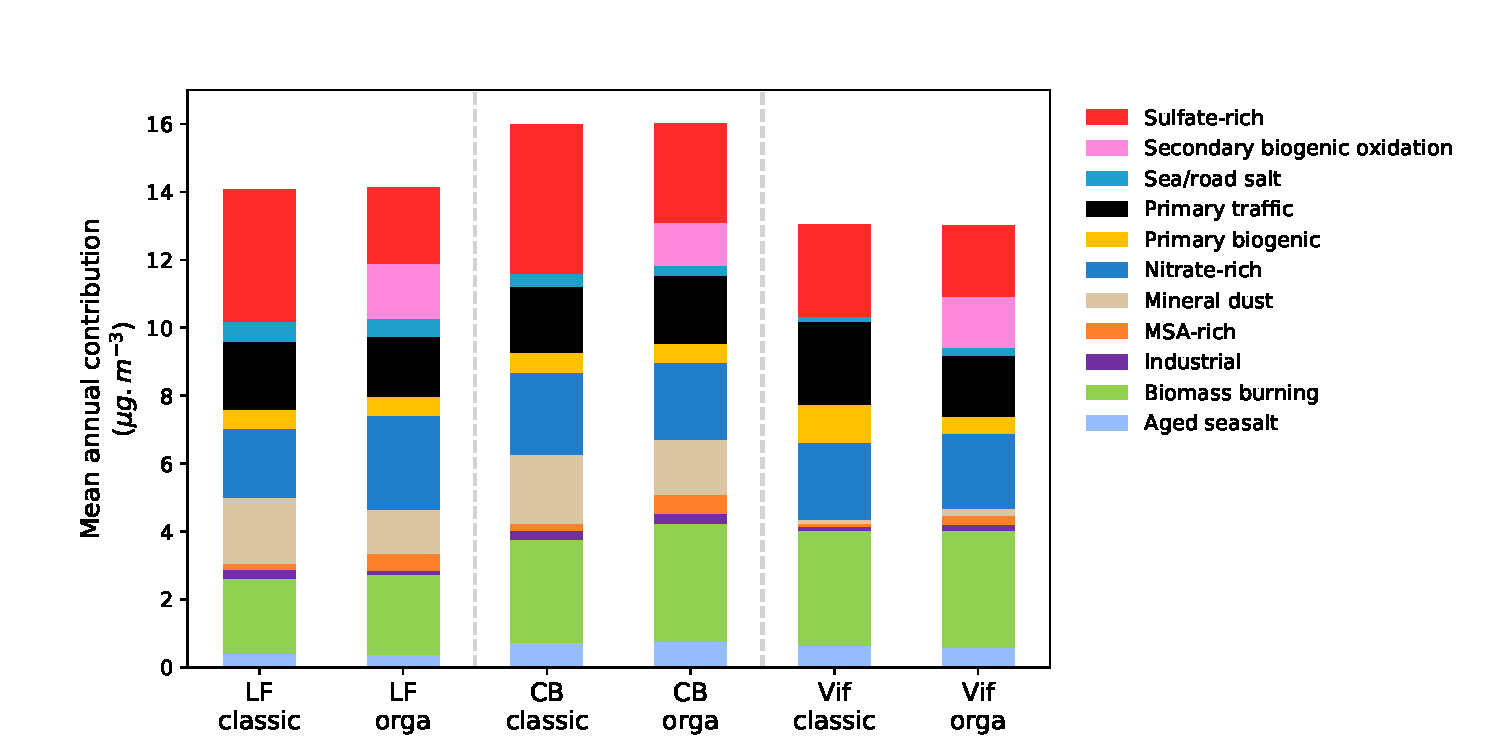
\includegraphics[width=1\linewidth]{chapter03/borlaza/Comparison_orga-woOrga_absolute.pdf}
    \caption{Comparaison des contributions annuelles des différents facteurs aux \PMdix{}
    pour les 3 sites entre les PMF classiques et organiques.}%
    \label{fig:chapter03/borlaza/Comparison_orga-woOrga_absolute}
\end{figure}

\subsubsection{Conclusion}%
\label{ssub:conclusion_organique}

Ainsi, en plus des conclusions sur les sources de PM et la variabilité fine échelle, qui
sont abondamment discutés dans l'article et rapidement rappelé ici, cette étude
multi-sites sur le bassin de la métropole grenobloise nous permet les conclusions
suivantes :
\begin{itemize}
    \item La variabilité des sources de \PMdix{} à l'échelle d'une moyenne métropole est
        relativement faible et les sites de fond urbain sont suffisamment représentatifs
        de l'ensemble de la métropole.
    \item La cellulose semble présenter un cycle saisonnier, mais des variabilités
        importantes à cette échelle spatiale sont également observées, indiquant très
        certainement des sources très locales de ce composé.
    \item Les phénomènes d'oxydation secondaires de la matière organique émise par les
        phénomènes biologiques (terpènes…) peuvent être ``capturés'' par une PMF sur
        filtres, notamment grâce au 3-MBTCA et à l'acide pinique.
\end{itemize}

Méthodologiquement, l'ajout de nouveaux traceurs spécifiques permet, même sur une solution
à 10 facteurs, de mieux séparer certains facteurs. Notamment, le 3-MBTCA et l'acide pinique
permette une meilleure estimation du facteur inorganique secondaire \textit{suflate rich}
qui était jusqu'alors un mélange entre de l'inorganique et de l'organique.
Cependant, l'ajout de la cellulose, présentant pourtant un signal unique, ne permet pas
l'identification d'un nouveau facteur dans la solution présentée ici. En revanche, lors de
nos essais sur cette PMF, nous avons expérimenté plusieurs incertitudes pour cette espèce,
et un ``seuil'' aux alentours de 15\% d'incertitude fait basculer la solution entre 11 et
12 facteurs, faisant apparaître un nouveau facteur très incertain statistiquement,
comportant la majorité de la cellulose.

Aussi, et dans la suite de la discussion de la section précédente
\ref{ssub:synthèse_grande_échelle_de_la_climatologie_des_polyols}, l'identification d'un
facteur d'oxydation secondaire en été ne change pas la contribution du profil primaire
biogénique, ce qui indique que ce facteur est suffissament contraint et bien déterminé par
ces espèces chimiques.

\clearpage

\section{SOURCES}%
\label{sec:sources}

\subsection{Introduction}

Les travaux présentés précédemment nous apprennent que les solutions d'une étude PMF sont
très dépendant des variables utilisées. Ainsi, il est compliqué de comparer 2 PMF
réalisées en définitive avec des méthodologies différentes.

Le projet SOURCES de l'ADEME avait pour ambition d'établir une synthèse nationale des
sources de PM, à travers des approches site-recepteurs --et donc PMF-- afin être au plus
près des observations de terrains.
Ainsi, 15 sites d'études ont été sélectionnés, reflétant la diversité des environnemnets
de la France métropolitaine, pour établir une méthodologie harmonisée d'étude PMF :
\begin{itemize}
    \item estimation des incertitudes communes,
    \item même espèces chimiques sélectionnées,
    \item même contraintes appliquées au modèle,
    \item estimation des incertitudes,
\end{itemize}
et ainsi établir une phénoménologie des sources de PM à l'échelle nationale.
Le rapport \cite{favezTraitement2017}, établi grâce au post-doctorat de Dalia Salameh,
décrit en détail la méthodologie utilisée ainsi que les profils et contribution
temporelles obtenues.

Dans cette partie, la comparaison géochimique des différents facteurs est discuté ainsi
que la variabilité de leurs incertitudes.

\begin{tcolorbox}[colback=red!5!white,colframe=Melon,title=Note]
    Le travail de recensement et d'établissement de cette méthodologie a été conduit lors
    du post-doctorat de Dalia Salameh, et a conduit à l'écriture du rapport 
    \cite{favezTraitement2017} (Français). Ce travail a été poursuivi durant ma thèse,
    notamment sur la partie concernant la comparabilité et variabilité des profils
    chimiques, et a été valorisé dans le papier \cite{weberComparison2019}, présenté ici.
    Le complément d'information est disponible sur \url{http://pmsource.u-ga.fr} et en
    annexe~\ref{annexe:SOURCES_SI}.
\end{tcolorbox}

\begin{tcolorbox}[colback=red!5!white,colframe=Melon,title=Note]
    Devant la quantité de donnée générée par cette étude, j'ai mis en ligne un site web,
    servant entre autres de complément d'information à l'article, mais aussi permettant aux
    utilisateurs d'explorer eux-mêmes l'entièreté des solutions obtenues (profils
    chimiques, contributions, incertitudes, deltaTool…) : \url{http://pmsource.u-ga.fr}.

    Au 20 juillet 2020, ce site a déjà été visionné par plus de 400 personnes provenant
    d'une vingtaine de pays, donc 30\% y sont revenus plusieurs fois.
\end{tcolorbox}

\subsection{Comparison of PM\textsubscript{10} sources profiles at 15 french sites using a harmonized constrained positive matrix factorization approach}%
\label{sub:article_SOURCES}
Article paru dans le journal \textit{Atmosphere} le 4 juin 2019 :

\begin{quote}
    Samuël Weber, Dalia Salameh, Alexandre Albinet, Laurent Y. Alleman, Antoine Waked,
    Jean-Luc Besombes, Véronique Jacob, Géraldine Guillaud, Boualem Mesbah, Benoit Rocq, Agnès
    Hulin, Marta Dominik-Sègue, Eve Chrétien, Jean-Luc Jaffrezo, et Olivier Favez. 2019.
    \textit{Comparison of \PMdix{} sources profiles at 15 French sites using a harmonized constrained
    Positive Matrix Factorization approach}. Atmosphere 10(6), p.310.
    \textsc{doi} : \href{doi:10.3390/atmos10060310}{https://doi.org/10.3390/atmos10060310},
    \textsc{url} : \url{https://www.mdpi.com/2073-4433/10/6/310}
\end{quote}


Une erreur typographique importante a été vue après publication : dans le tableau 
\textit{\textbf{Table~2.} Input variables and uncertainties used in the PMF analyses.}, la
valeur du coefficient $a$ pour les marqueurs organiques n'est pas de $0.01$ mais $0.10$.


\includepdf[pages=-,scale=0.9,pagecommand={\pagestyle{fancy}}]{chapters/sources.pdf}

\subsection{Conclusion}%
\label{sub:conclusion_SOURCES}

Des connaissances fines sur les provenances des espèces chimiques permet d'identifier les
sources prépondérantes de \PMdix{} à grande échelle lors d'étude PMF multi-sites.
Ces connaissances permettent aussi l'utilisation d'un ensemble de contrainte minimale
conduisant en l'amélioration des profils chimique PMF obtenus mais également de meilleurs
stabilité statistiques, tant en termes de diminution de l'erreur aléatoire (bootstrap) que
de diminution de l'ambiguïté rotationelle (displacment).
Enfin, la mise en place et l'utilisation d'une méthodologie harmonisée d'étude PMF permet
une comparabilité inter-sites à travers l'outil DeltaTool.

L'utilisation de cette méthodologie, incorporant des espèces organiques, permet non
seulement d'établir une phénoménologie des \PMdix{} à grande échelle spatiale, montrant
des variations saisonnières importantes des sources de PM, mais améliore également la
robustesse statistique --estimée par bootstrap et displacment-- et géochimique
--similitude des facteurs et présence à large échelle spatiale--, y compris pour des
facteurs peu courant dans la littérature comme les émissions primaires biogéniques et le
MSA-rich.

Ces recherches permettront prochainement la comparaison entre modèle PMF, proche des
observations, et déterministe CTM, afin de comprendre et si possible d'améliorer, les
potentiels manquement dans les processus implémentés dans les CTM, et ce pour une large
gamme de conditions environnementales.

\section{Conclusion}%
\label{sec:conclusion_chap3}

\subsection{Résumé du chapitre}%
\label{sub:résumé_du_chapitre_3}

L'ajout de nouveaux traceurs spécifiques permet une meilleure estimation des profils
chimiques des différents facteurs PMF obtenues. 

Une nouvelle source primaire et une part du biogénique secondaire sont identifiées
respectivement grâce aux polyols (arabitol et mannitol) et MSA, avec une grande robustesse
statistique tant intra-site (faible incertitudes pour ce facteur) qu'inter-site (retrouvés
sur l'ensemble des études où ces espèces sont introduites, et fortes similitudes
géochimiques entre les différents profils sur différents sites mesurées par l'approche deltaTool).
Nous avons aussi montré que grâce à un traitement préalable du signal isotopique de
l'ammonium, il est possible d'attribuer le facteur inorganique \textit{Nitrate-rich} au
secteur agricole.
Enfin, une part secondaire de la matière organique peut efficacement être regroupée dans un
facteur d'oxydation secondaire par l'introduction du 3-MBTCA et de l'acide pinic.

Il est important de noter qu'à chaque ajout d'un nouveau traceur, seul un facteur,
jusqu'alors étant manifestement un mélange de différente sources ou processus, évolue.
C'est donc bien un raffinement des solutions et non une remise en cause des solutions
précédentes.

Finalement, la variabilité des profils chimiques intra- et inter-sites pour une étude
PMF harmonisée sur 15 sites différents montre qu'il est possible de réduire la part
subjective de l'expérimentateur tout en ne masquant pas les spécificités propres à chaque
site.

\subsection{Pistes de travaux futurs}%
\label{sub:pistes_de_travaux_futurs}

Si certaines espèces sont maintenant mesurées en routines à l'IGE (polyols et MSA),
d'autres sont encore utilisées à des fins de recherches et ne sont pas encore utilisable
à des fins opérationnelles. En effet, s'il est possible d'agir sur les émissions de
combustion de biomase ou liés au trafic routier mais également de savoir sur lesquels
il est difficile d'avoir une action (primaire biogénique), les facteurs organiques
secondaires sont difficilement attribuables à un ou des secteur·s d'activité·s. Cette
limitation propre aux facteurs secondaires peut être levée, comme nous l'avons vu avec
l'isotopie de l'ammonium, mais doivent faire l'objet d'études approfondies.

Aussi, d'autres espèces organiques peuvent être utilisées comme vu en introduction (HAP,
BNT, hopanes, alcanes…), et permettraient potentiellement une meilleure caractérisation de
plusieurs sources anthropiques (trafic, portuaire, industrielle…) ou liés aux débris végétaux.
À ce titre, une PMF sur La Paz (Bolivie) est en cours dans le cadre de la thèse de Valéria
Mardonez dans le groupe CHIANTI.

Cependant, l'ajout de nouveau traceur présentant un signal singulier ne suffit pas
nécessairement à la caractérisation d'un nouveau facteur, comme nous le pensions pour la
cellulose. L'estimation des incertitudes semble jouer ici un rôle prépondérant.
Afin d'en apprendre plus à ce sujet, 6 séries annuelles de prélèvement \PMdix{} et \PMdc{}
en Suisse ont été analysées à l'IGE et permettent une étude PMF incluant ces nouveaux marqueurs
organiques, et ce sur les 2 fractions des PM. Cette étude est en cours par Stuart Grange de
l'EMPA, avec lequel j'interagis régulièrement sur ces questions.

% Question : SPECIEUROPE et contrainte trop fortes sur certains profils ?

Enfin, la ``filtrothèque'' construite aux fils des ans à CHIANTI ouvre la voie à une
étude PMF de 2011 à 2020 sur site de l'OPE, pour la fraction \PMdix{} et \PMdc. Une
telle série de prélèvement permet l'analyse tendancielle des facteurs PMF et donc
l'estimation de l'efficacité des différentes mesures de protection de la qualité de l'air
de la dernière décennie. Les résultats préliminaires semblant notamment indiquer une baisse
progressive des émissions liés au trafic routier, également retrouvé par la tendance à
la baisse des émissions d'EC observées par les différentes campagnes ACTRIS.
\todo{mettre la figure}

\todo{trouver une facons de dire que depuis n ans, j'ai pas mal d'expertise et que
j'encadre stagiaire/début de thèse sur la formation PMF.
Travaux : bcp de chose, pas tous seul mais en groupe, mais moi encadrement et formation.
}

%
% Limitation : 
% - espèce trop réactive ? (oxalate ?)
% - résolution temporelle \cite{wangSource2018}
% - PMF multisite ? \cite{pandolfiLongrange2020,daiImproving2020}

